%%%%%%%%%%%%%%%%%%%%%%%%
%% Sample use of the infthesis class to prepare a thesis. This can be used as 
%% a template to produce your own thesis.
%%
%% The title, abstract and so on are taken from Martin Reddy's csthesis class
%% documentation.
%%
%% MEF, October 2002
%%%%%%%%%%%%%%%%%%%%%%%%

%%%%
%% Load the class. Put any options that you want here (see the documentation
%% for the list of options). The following are samples for each type of
%% thesis:
%%
%% Note: you can also specify any of the following options:
%%  logo: put a University of Edinburgh logo onto the title page
%%  frontabs: put the abstract onto the title page
%%  deptreport: produce a title page that fits into a Computer Science
%%      departmental cover [not sure if this actually works]
%%  singlespacing, fullspacing, doublespacing: choose line spacing
%%  oneside, twoside: specify a one-sided or two-sided thesis
%%  10pt, 11pt, 12pt: choose a font size
%%  centrechapter, leftchapter, rightchapter: alignment of chapter headings
%%  sansheadings, normalheadings: headings and captions in sans-serif
%%      (default) or in the same font as the rest of the thesis
%%  [no]listsintoc: put list of figures/tables in table of contents (default:
%%      not)
%%  romanprepages, plainprepages: number the preliminary pages with Roman
%%      numerals (default) or consecutively with the rest of the thesis
%%  parskip: don't indent paragraphs, put a blank line between instead
%%  abbrevs: define a list of useful abbreviations (see documentation)
%%  draft: produce a single-spaced, double-sided thesis with narrow margins
%%
%% For a PhD thesis -- you must also specify a research institute:
\documentclass[msc,ilcc,oneside]{infthesis}

%% For an MPhil thesis -- also needs an institute
% \documentclass[mphil,ianc]{infthesis}

%% MSc by Research, which also needs an institute
% \documentclass[mscres,irr]{infthesis}

%% Taught MSc -- specify a particular degree instead. If none is specified,
%% "MSc in Informatics" is used.
% \documentclass[msc,cogsci]{infthesis}
% \documentclass[msc]{infthesis}  % for the MSc in Informatics

%% Master of Informatics (5 year degree)
% \documentclass[minf]{infthesis}

%% Undergraduate project -- specify the degree course and project type
%% separately
% \documentclass[bsc]{infthesis}
% \course{Artificial Intelligence and Psychology}
% \project{Fourth Year Project Report}

%% Put any \usepackage commands you want to use right here; the following is 
%% an example:
\usepackage{url}
\usepackage{natbib}
\bibliographystyle{apalike}

\usepackage{graphicx}
\graphicspath{ {graphics/} }
\usepackage[space]{grffile}

\usepackage{titlesec}
\setcounter{secnumdepth}{6}
\setcounter{tocdepth}{6}

\usepackage{listings}
\lstset{
basicstyle=\small\ttfamily,
columns=flexible,
breaklines=true
}

%% Information about the title, etc.
\title{Channel Shift - using data analysis to improve service delivery at the City of Edinburgh Council}
\author{Michal Wasilewski}

%% If the year of submission is not the current year, uncomment this line and 
%% specify it here:
% \submityear{1785}

%% Optionally, specify the graduation month and year:
% \graduationdate{February 1786}

%% Specify the abstract here.
\abstract{%
    This project conducts data analysis activities which aim at providing insights that can drive improvement of services delivered by the City of Edinburgh Council (CEC). Business Intelligence (BI) tools are used together with design methods and practices. The design process is described using Double Diamond model. The results provide CEC employees with a better understanding of the needs of citizens.
}

%% Now we start with the actual document.
\begin{document}

%% First, the preliminary pages
\begin{preliminary}

%% This creates the title page
\maketitle

%% Acknowledgements
%\begin{acknowledgements}
%Many thanks to my mummy for the numerous packed lunches; and of course to
%Igor, my faithful lab assistant.
%\end{acknowledgements}

%% Next we need to have the declaration.
\standarddeclaration

%% Finally, a dedication (this is optional -- uncomment the following line if
%% you want one).
% \dedication{To my mummy.}

%% Create the table of contents
\tableofcontents

%% If you want a list of figures or tables, uncomment the appropriate line(s)
% \listoffigures
% \listoftables

\end{preliminary}

%%%%%%%%
%% Include your chapter files here. See the sample chapter file for the basic
%% format.

%% Sample chapter file, for use in a thesis.
%% Don't forget to put the \chapter{...} header onto each file.

\chapter{Introduction}

Over the last few years, the School of Informatics has been collaborating with the City of Edinburgh Council in the area of open data in initiatives such as the Smart Data Hack and the Council's EdinburghApps hackathons. In the context of Edinburgh Living Lab, this relationship has broadened into investigating other areas of data science, and new kinds of collaboration. My MSc project is taking place within this context, and is focussing on bringing analytic techniques to bear on Customer Relationship Management (CRM) data that has been collected by the Council over the last year.

	\section{Context}

As one of the fastest growing local authority areas in Scotland, Edinburgh is facing an ever increasing demand for Council services, outstripping the funds available to meet this demand. There are a number of projects on-going in the Council that try to address the resulting challenges, one of which aims to improve the way that Council interacts with residents, particularly in terms of dealing with complaints and reports of problems. At the moment, citizens can communicate with the Council using multiple "channels": email, web forms, mobile apps, phone, post and face-to-face conversation. So-called "Channel Shift" is the policy of encouraging residents to use web forms in preference to other communication channels. Some other objectives include informed design of interfaces and web-forms, increase in the use of digital channels and decrease in traditional channels for selected transactions. The Council has been recently building capacity to collect data and use sophisticated tools for managing and integrating it. This project is hoping to contribute to internal resources for extracting business insights from analysing this data. More broadly, I hope that my research will help the Council to ensure that transactions initiated via digital channels are dealt with effectively, as well as contribute to creating "success stories" and know-how within the Council.

	\section{Objective of the project}

Using analysis of CRM data provide insights about the delivery of CEC services to the residents of Edinburgh. These insights should serve as guidelines for improvement of existing interactions between the Council and citizens as well as help in implementation of transactions for services which are not supported over digital channels yet.

	\section{Thesis structure}

The first part of this thesis is devoted to providing a theoretical background to the work undertaken. User Centred Design (UCD) is a concept in design that has played a major role in building interfaces to computational systems over the last three decades. It encompasses a set of tools and practices used when designing interfaces and services (e.g. web-form, application interface). It is described here providing a historical context and modern developments in related fields. Human Centred Design, which is a broader term, not only considers the person as a user (as it is in the case of UCD), but also as a human. Design Driven Innovation was proposed by Roberto Verganti and it is expanding design strategies and methods (e.g. UCD) to include innovation in meaning. Data-driven design is a practice of designing with the use of data driven rather than human driven (ethnographical) methods. Double Diamond methodology is a model of practicing design (conducting design related activities) which is claimed to be describing a universal framework for a design process, not limited to any particular field.

The second part is describing the work undertaken and is divided into four phases in accordance to the Double Diamond model. The Discover phase describe the initial, exploratory activities in the project. The Define phase narrow down the scope, finishing with three defined objectives. The Develop stage is describing the process of implementation and results. The Deliver part covers delivering the results to the clients and feedback received.

The last two parts are dedicated to evaluating the project and drawing conclusions. Tools used in the process are evaluated, the work undertaken and methodology used. 
%% Sample chapter file, for use in a thesis.
%% Don't forget to put the \chapter{...} header onto each file.

\chapter{Background}

	\section{User Centred Design}

		\subsection{Introduction to User Centred Design}

The term User Centred Design was coined and popularized by Donald Norman's research group in the 1980s. Two influential books were published in that time which he co-authored: "User centered system design" \citep{norman1986user} and "The psychology of everyday things" \citep{norman1988design}. UCD is sometimes referred to as User Centred System Design (UCSD). This ambiguity comes from the definition of UCD not being agreed upon for many years \citep{Gulliksen2003}.

User Centred Design (UCD) is a broad term that describes both a philosophy and a set of tools used during the design process \citep{norman1986user, norman2013design}. At its core, it gives central role to the needs and limitations of the user. The level of involvement of the user in the design process may vary, but the fundamental difference compared to other approaches is that decisions are driven by a very deep understanding of users' needs (or even by users themselves). It is not limited to interface optimisation and often means working closely with users already at definition stage where they help in the problem identification. Fundamentally, UCD tries to "focus on usability throughout the entire development process and further throughout the system life cycle" \citep{Gulliksen2003}.

The need for "people oriented" interfaces was already recognized in the early days of computers \citep{ritter2014foundations, nickerson1969man}. Voices of concern were raised that product development methods used at the time were more suitable for big, labour intensive projects and were failing with sophisticated devices which focus on usability \citep{greenbaum1993design, robert1965new}. In 1960s and 1970s there were a number of fields in academia concerned with designing more human friendly devices and processes, but they were applied with varied success. What made UCD so effective was that it "focused on the needs of the user, on activity/task analysis as well as a general requirements analysis, carrying out early testing and evaluation, and designing iteratively." \citep{ritter2014foundations}. It also emphasized the involvement of the user in the design process instead of treating him purely as a consumer of the product. This has been a paradigm shift that was particularly uncomfortable for managers in the United States who were reluctant to hand over the decision making power \citep{greenbaum1993design}.

UCD has changed over the years.  Initially UCD was focused on command-line tools, but as computers got more widespread and their interfaces became more sophisticated, it started growing in importance and played a different role. With Graphical User Interfaces (GUI) it was focused on layouts and optimisation and with nowadays proliferation of computational systems, UCD design is considering things like personal preferences or social and cultural impact of the device \citep{ritter2014foundations}.

		\subsection{Human Centred Design}

Human Centred Design (HCD) is a broader term that puts humans at the centre \citep{ritter2014foundations, Earthy2001, iso199913407, 1_kurosu_2011}. This means taking into consideration the entire context of the situation in which the product will be used and the human aspects of it. It is considered more interdisciplinary than UCD and is described in many standards \citep{Bevan2001} such as ISO 13407:1999 \citep{iso199913407} and more recently 9241-210: 2010 \citep{dis20099241}. UCD is considered by some as being too much focused on solving a goal-directed, technological problem and limited by considering people solely as users of the system without looking at the organisational goal or counteracting possible adverse effects of use on human health, safety and performance \citep{gasson2003human, gill1996foundations, Bevan2001}. UCD and HCD are not synonyms and HCD does not necessarily imply using UCD methods \citep{Earthy2001, Maguire2001, 1_kurosu_2011, ritter2014foundations}. 
		
		\subsection{Design Driven Innovation}

A recent perspective that is broadening the definition of design to include a reconstructionist \citep{chan2005blue} or social-constructionist \citep{Prahalad2000} view of the market is Design Driven Innovation \citep{Liem2011, verganti2013design}.   

In his book "Design driven innovation: changing the rules of competition by radically innovating what things mean" Roberto Verganti introduces the concept of Design Driven Innovation \citep{verganti2013design}. In his opinion, most organisations understand and use design in two ways: making things beautiful and stylish and having a profound (and thus accurate) understanding of user needs. Innovations coming from these two, beauty of the product and user needs (which is an embodiment of User Centred Design), are in his opinion insufficient for market differentiation and have become so common that they are a norm rather than exception. Verganti argues that what is needed (together with the first two) is a third use for design which is a radical innovation in meaning.

His research reveals that recent management literature focuses on technological innovation and what effect it has on an industry. What is also very well covered is looking beyond features and understanding the meanings behind them - what emotions drive people to buy products. However, the silent assumption is, he continues, that meanings are not a subject of innovation. He proposes a third strategy for design which is innovation in what meaning things can carry.

The author brings and analyses dozens of examples to help better understand design-driven innovation such as:

\begin{itemize}
\item Artemide, Italian lamp manufacturer, created a lamp that is no longer a source of light, but an object that has influence on people's mood. Effectively, by providing a device that can change intensity and colour of the light you are enabling people to control their mood and the product becomes an element of well-being.

\item The MP3 players were present before iTunes, but it was a change in how to think about music brought by Steve Jobs that revolutionised the industry. Many executives and lobbing groups stubbornly focused on enforcing copy-protection, whereas Apple enabled users to buy a single song instead of an entire album, taste and mix music, create personal playlists.

\item Anthropomorphism in the shape of kitchen appliances brought by Alessi, turned equipment into objects of affection, things you bond with, "teddy bears for adults" \citep{verganti2013design}.

\item Apple's move to release a notebook without an optical drive was considered a bold one, but Steve Job had an understanding of what cloud computing and wireless connectivity meant - constant access to vast amounts of data and thus no use for CDs/DVDs.
\end{itemize}

The author also provides a structured framework for thinking about innovation in meaning and deploying it in an organisation. Design Driven Innovation extends beyond User Centred Design, but does not discredit it.

	\section{Data-driven design}
	
Data-driven design is an emerging field of study that gained popularity with the digitization of our world and in particular with what is known as big data. The premise of data-driven design is an additional layer of perception provided by data collection and processing, previously unavailable to humans. Although the practices of data-driven design are far from being well established, more and more voices are being raised that consider it a very viable tool when used properly with other methods \citep{Neirotti2014}.
	
		\subsection{What would a cup say if it could speak?}

Data can be used to drive the design of many things. Common areas of use of data-driven design in Informatics include websites (web analytics) or mobile apps. A designer can change the layout of a website and in real time analyse what impact on the behaviour of the user it has \citep{CSIRO2015}.

However, computational systems are being used for much more than just reading websites. Vizie is a tool analysing social media feeds and it is able to inform government institutions about a failure of a service, provide situational awareness in emergencies or simply help being in touch with citizens by informing about major topics of the day \citep{CSIRO2015a}. In one case, social media is actually the main, preferred way of communicating with a government institution - for better or for worse \citep{MITMediaLab2015}.

The Internet of Things (IoT) is another case of digitization entering our lives. We are instrumenting objects in our surroundings "giving them a voice". IoT devices will generate a lot of data about their users and the devices themselves. Vessyl is an IoT cup designed to be part of a bigger health and wellness ecosystem. It traces the nutritional value of liquids consumed by the user \citep{MarkOne2014}. Interesting questions arise from the designers' perspective with the emergence of such devices. What impact on the design of the cup do the consumption habits of its users have? If the cup could capture detailed data about its usage patterns - location, acceleration, angle of tilt - could it suggest a better design (e.g. thinner, taller, rounded edges)? Maybe the cup would tell us something else, unrelated to the drink, something that we cannot think of simply because we are humans?

This vast amount of data captured in different areas of people's lives provides a lot of opportunities for generating design insights. It is important to stress that having data by itself is not sufficient. It is what follows - data analysis - that makes all the difference and that is where uncharted territories are.

			\subsubsection{What is big data?}

There are many definitions of what Big Data is and in some cases not only do they differ, but even stand in contradiction. This might be due to the fact that early cases of use of the term happened in different fields \citep{demchenko2014defining, Ward2013}. Most commonly, Big Data is associated with data storage and data analysis, which in themselves are not new concepts at all. A description that is widely accepted as fundamental in coining the term Big Data is the "3 Vs" definition provided by Gartner in 2001 \citep{douglas20013d, Ward2013}. Since then, the "Vs" description has been used and expanded (to "5 Vs") by many \citep{McAfee2012, minelli2012big, demchenko2014defining, NIST2015}.

The "5Vs" of big data are as follows:
\begin{itemize}
\item Volume - 90\% of world's data was generated over the last two years; by some, big data is considered when dealing with volumes over peta bytes ($10^{15}$)

\item Velocity - more data being received than can be processed using "traditional" data analysis approach; you receive more information than you can process before a decision has to be made; processing of real-time data streams is becoming essential

\item Variety - different types of data are being accessible (structured data, sensory data, social media data, voice recordings, photos, videos)

\item Veracity (validity) - lack of control over quality and accuracy which leads to inconsistencies and incompleteness

\item Value - how to get value out of data
\end{itemize}

		\subsection{Data Analysis}
		
Data analysis is a process of cleaning and inspecting data using tools such as modeling, reasoning, processing and visualising. It is a complex activity that can be done with different objectives in mind, e.g. discovering relations, supporting decision making by delivering business insights, designing systems and processes, delivering services and products.

Due to the amount of data that is usually processed when doing data analysis as well as complexity of this task, Artificial Intelligence (AI) algorithms are deployed. Fields of AI that are most often used for data analysis include Machine Learning (ML) and Pattern Recognition (PR) \citep{bishop2006pattern}. They have many uses with structured and unstructured data. Some of those relevant in this context include: text/speech recognition, customer choices analysis, usage patterns analysis, decision support systems involving judgment, load forecasting, marketing and sales \citep{witten2005data}.
			
			\subsubsection{Business Intelligence}
Another Data Analysis technique is Business Intelligence (BI). It is focused on delivering business insights. The term Business Intelligence was coined by Howard Dresner from Gartner Group in 1989. It describes a set of data-driven tools and practices that emerged from Decision Support Systems (DSS) which went through a time of intense development in 1980's \citep{power2008decision}. BI has been a very popular and dynamic field in recent years which is attributed to, among many others, "more turbulent business environments" and higher demands for profitability \citep{sacu2010bidm, power2008decision, baars2008management}. A range of BI tools that are becoming popular recently are the user-driven solutions which promote "self-service" as opposed to dependence on IT department's involvement \citep{IBM2015a, Qlik2015, Microsoft2015, imhoff2011self}.

The goal of BI is to unveil valid risks and performance indicators, through the means of interpretation (processing) of large volumes of data, in order to support managers on all levels: strategic, tactical and operational \citep{baars2008management}.

There are numerous models describing BI maturity. In general, they take into consideration the following concepts: deployment, use and impact of BI in an organisation \citep{Lahrmann2011}.

Currently most widely used tools within BI are reporting, data mining and Online Analytical Processing (OLAP). In many areas this is insufficient as a lot of data is not numerical or otherwise referred to as unstructured, e.g. voice transcripts, comments, e-mails, documents. This is especially true for analysing data about interactions with customers such as data from Customer Relationship Management (CRM) systems \citep{baars2008management}. There are different approaches and frameworks for building systems that incorporate both data types. In general, they can either process unstructured data to extract from it information in a more structured way (e.g. text processing), present both data types next to each other without processing unstructured data (e.g. show all e-mails relevant to a performance indicator to allow human to understand the situation) or anything in between.

		\subsection{Smart Cities}
Data is considered to be an essential asset in Smart Cities (SC). They make use of it and in many initiatives it plays a major role in the design and operations of city services.

SC try to improve the lives of citizens by creating more sustainable and more efficient urban environment for people to live in \citep{geertman2015planning}. Using technology-based solutions they try to address some of the challenges faced by metropolitan areas \citep{Neirotti2014}. Although there is no clear definition yet of what a SC is, it is widely accepted that Information and Communications Technologies (ICT) play a major role in SC by acting as their "nervous system" \citep{Neirotti2014, geertman2015planning}. Data about different aspects of functioning of the city will be collected, analysed and acted upon in real time. However, ICT capabilities by themselves are not sufficient and have to be matched with adequate human and organisational capital in order to enable cities to act accordingly.  Some research suggest that globally, initiatives within SC are highly diverse and depend heavily on the cultural and socio-economic background of the geographical region making it non trivial to find commonalities, but with time a few archetype models will emerge \citep{Neirotti2014, geertman2015planning}. The highest number of initiatives in area of SC has been observed in "Natural resources and energy" and "Transport and mobility" \citep{Neirotti2014}.

Transportation in Nairobi, Kenya using semi-formal mini-buses has been a subject of a project that used GPS data to improve route planning and way finding \citep{klopp2015leveraging}. The location data was not acquired through telecommunications operators, but was willingly shared by users via a smartphone app. It was made public in GTFS format and processed using open-source tools such as Open Trip Planner \citep{klopp2015leveraging}. It is an example of "bottom-up" approach in which citizens are empowered (Open Data) and supported by local authorities to act and improve their city \citep{Neirotti2014}.

In 2012 the New York City Council has approved a law requiring all city agencies to open their data by 2018. One of the agencies helping in this process is Mayor's Office of Data Analytics (MODA). MODA is responsible for initiatives within five categories: Supporting Operations, Citywide Data Sharing, Disaster Response and Resiliency, Economic Development, Open Data. They are offering courses to other City government employees about data and tools available to them and are also promoting data driven decision making \citep{NYCMODA2014}. One interesting project in New York City is called "Hudson Yards Redevelopment Project" in which an entire part of the city will be built from scratch. It will be collecting information about air quality, pedestrian traffic, energy production and consumption. It will have a trash-disposal system to remove waste via underground pneumatic tubes.

	\section{Double Diamond}
	
"Double Diamond" is a model of the design process developed by the UK Design Council \citep{council2007eleven, council2005double}. It is a result of a qualitative study of practices in companies focused on innovation and it describes the commonalities in the creative activities that can be observed among designers regardless of the field they are working in. The model divides the design process into four phases as pictured in Figure 2.1. Each of those phases is focused on a different objective and involves methods which are characteristic to that stage.

\begin{center}
  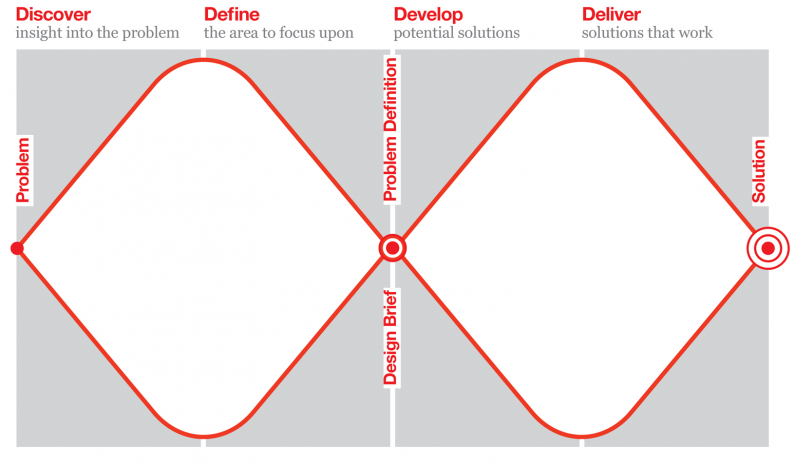
\includegraphics[width=1.0\textwidth]{Double-Diamond-A3-for-publication-A-2000px_1.png}
  \captionof{figure}{Four phases of the design process as defined by the Double Diamond model \citep{council2005double} }
\end{center}

		\subsection{Discover}

At this stage the attitude adopted is of openness in terms of thoughts and ideas. All ideas are welcome, different perspectives are nurtured and every direction has the potential to be valid. This thinking is typical at the beginning of the project. Designers try to remain as open as possible so that their own perspectives do not limit creativity. This helps in noticing things that might matter, clues about what would make the situation better especially that it might be something unexpected or not identified.

Some of the activities used at this stage include:
\begin{itemize}
\item Observation
\item User diaries
\item Being your users
\item Brainstorming
\item Choosing a sample
\item Quantitative surveys
\item Fast visualisation
\item Secondary research
\item Hopes and fears
\item Market research
\item User research
\item Managing information
\item Design research groups
\end{itemize}

		\subsection{Define}
		
Second phase is trying to make sense out of all the information collected. It is focused on identifying causalities, narrowing down insights and establishing the main challenge which will be addressed. It takes into consideration limitations of the project in terms of what is feasible given the time and resources. Selection and discarding of ideas takes place here as well. It starts with numerous concepts and ideas and finishes with a clear definition of the problem and a list of actionable tasks.

Activities at this stage often involve:
\begin{itemize}
\item Focus groups
\item Assessment criteria
\item Comparing notes
\item Drivers and hurdles
\item Customer journey mapping
\item Project development
\item Project management
\item Project sign-off
\end{itemize}

		
		\subsection{Develop}
		
This stage involves intense creation, prototyping and testing. It takes the results of the previous phase as a "design brief" and uses it as a framework for the development process. Iterating is very important in order to improve and refine the prototypes as well as concepts. Attitude of trying and failing ensures the space for testing different implementations using different techniques and thus finding the best one. Some of the tools used are similar to Define stage, but here they are focused on bringing a product ready for production.

Typical to this stage are:
\begin{itemize}
\item Character profiles
\item Scenarios
\item Role-playing
\item Service blueprints
\item Physical prototyping
\item Multi-disciplinary working
\item Visual management
\item Development methods
\item Testing
\end{itemize}		
		
		\subsection{Deliver}

The last phase is when the product is being finalised, produced and launched. Here it is mass produced, checked before release and delivered to the user. Feedback mechanisms should be in place which will improve the product itself, but also methods and practices used in the process of creation of it.

Characteristic to this phase are the following activities:
\begin{itemize}
\item Phasing
\item Final testing
\item Evaluation
\item Feedback loops
\item Methods banks
\item Approval
\item Launch
\item Targets
\end{itemize}




%% Sample chapter file, for use in a thesis.
%% Don't forget to put the \chapter{...} header onto each file.

\chapter{Description of the work undertaken}
	\section{Discover}
	
During the discovery phase of the project the objective was to become familiar with the CEC environment, i.e. find out what tools are available and how they are being used and gather information about how to best contribute to the organisation. This was to be done while staying as open as possible, allowing any influences or ideas.

At the beginning of the project I had no knowledge about the operations within the Council or which departments would be involved. Some of the questions I wanted to answer included:
\begin{itemize}
\item Are there any activities in the Council similar to the scope of the project (or were there any in the past)?
\item Who would benefit from it and how to give those stakeholders an opportunity to be involved?
\item What questions (in terms of "channel shift") are not answered in the Council?
At what level of abstraction should the analysis be conducted?
\item What IT systems/tools can be used in the project?
\item Who has the necessary understanding of the infrastructure and activities on the architectural level?
\item What else do I not know?
\end{itemize}

		\subsection{Meetings at the Council}
		
Initially the contact person from the Council was Sally Kerr. In response to my questions she arranged a meeting with an enterprise architect Neil Dumbleton. The purpose of the meeting was to give me an opportunity to ask questions regarding organisational structure as well as context of the project.

As it turned out, it was a first meeting in a series. There was no formalised documentation or central place with knowledge about on-going projects that was made available to me. As a result, personal meetings were the only way to understand activity in the Council. Moreover, it was only thanks to goodwill of many employees at the City of Edinburgh Council that this was possible.

The figure 3.1 shows all people I interacted with during the entire project. Connections between different actors represent how I got to know them. Circles with coloured backgrounds highlight people who I spoke with in this phase. People marked with two big ovals show people who I spoke with in the next phase. Level of a circle does not reflect a position in the Council's structure - it is used solely for increasing legibility of the diagram.

\begin{center}
  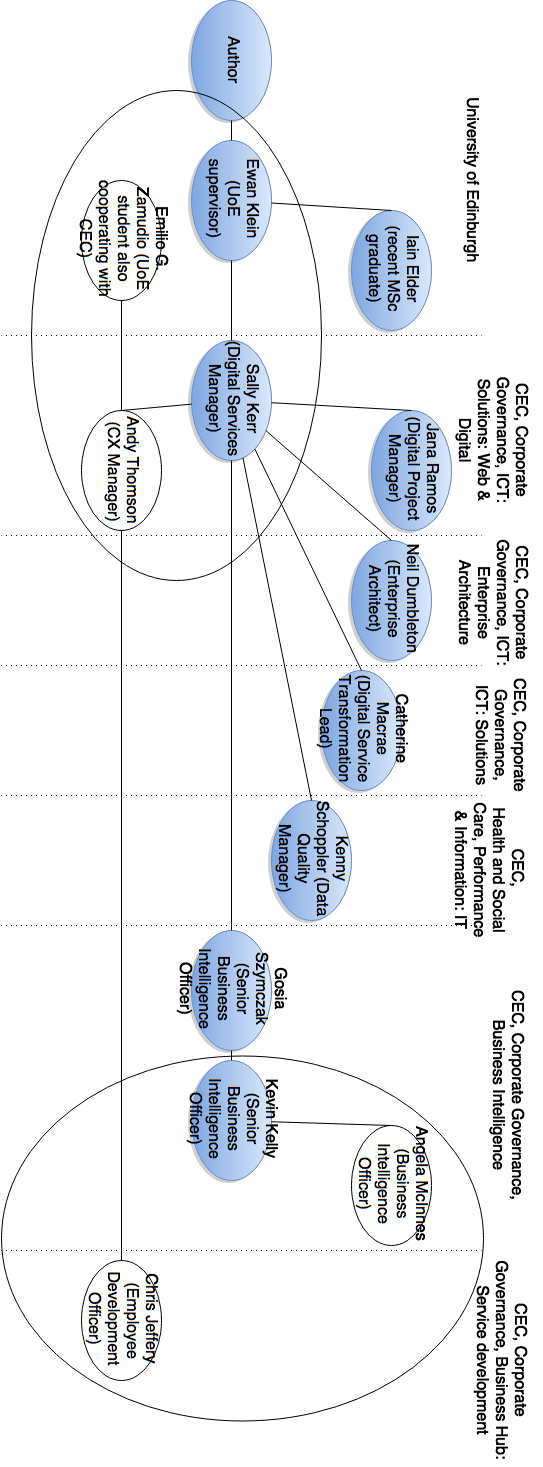
\includegraphics[height=0.95\textheight]{Discovery_phase_people.png}
  \captionof{figure}{CEC employees involved in the project.}
\end{center}


From these meetings and discussions I gained an initial understanding of the situation at CEC. There was a big effort within the Council aiming at transforming the way services are being delivered and "Channel Shift" was a part of it. The outsourced ICT services in the Council were delivered by British Telecom starting from 2001 and the contract was set to end in 2016. In order to find a new service provider under revised conditions, a public tender was being held during the writing of this thesis. It considered "Channel Shift" as one of the significant enhancements of the Council's operations. Final report suggesting the best bidder was submitted by the Finance and Resources Committee on third of August 2015 \citep{FinanceandResourcesCommittee2016}.

In summer 2014 a new CRM system was introduced which was replacing the old one called Capture. The deployment of the new system was part of the transformation efforts. It was used to capture information about all interactions with citizens and in some cases it meant that entries did not have all the values specified (due to the nature of an inquiry). The incompleteness of entries did not make them useless as they could still inform about things like level of use. The data captured has not been analysed from the angle described in this project (socio-economic insights) and it was confirmed that such analysis would be useful for the Council.

The transformation within the Council was also trying to centralise Business Intelligence capabilities. The BI department had a number of responsibilities and systems. One of those systems was called IBM Cognos. It was fully operational and a number of reports were generated and delivered to other stakeholders. However, the scale of deployment was still unclear and many departments were still figuring out the role the system would play in their operations. Many services required more digitisation and given the strategy, they could potentially use Cognos in the process. CRM data was an example of a dataset that was promising in providing valuable business insights.

Considering the above, the project would develop a piece of work that would increase know-how within the Council (in terms of using data analysis for designing services and interfaces), provide a "case study" and directly deliver business value to the organisation. The tools and datasets that could be used are described in the following sections.

		\subsection{CRM data}
		
The new system used at the Council was called RightNow and was provided by Oracle. It was a cloud service and the data in the system was available to CEC employees after registration (with staff number) and installation of the interface. The database consisted of a number of tables, e.g. "Answers" which was a "knowledge base for consultants". The table used in the project was "Incidents" and it contained information about transactions initiated by citizens (issues reported by them through all channels). This choice was dictated by the scope of the project - de facto by preferences of the clients who were interested in better understanding of the usage patterns of citizens.

Unique Property Reference Number (UPRN) was a number uniquely identifying a household in Edinburgh and thus a person (or a family). It was removed from all figures due to privacy concerns. The "Incidents" table had a column named UPRN which provided information about who reported the issue. The Mosaic personas (introduced in the next section) were also using UPRN making it possible to link the two datasets. The table had dozens of columns containing information about things like channel used to report the issue, postcode where it was reported, date, Service Level Agreement (SLA).

The table provides also means for tracking activity across different channels. Some enquires are just general questions and as a result, many entries do not have all values filled in. This enriches the dataset giving a fuller picture of what is happening, i.e. keeping a trace of all enquires.		
		
		\subsection{Mosaic UK Consumer and Demographic data}
		
Mosaic is a dataset created by Experian - credit reference agency. It provides insights about lifestyles and preferences of people across the United Kingdom. Depending on the version of the dataset, it identifies 56 types of households which are categorized into 14 general groups:
\begin{itemize}
\item A - City Prosperity
\item B - Prestige Positions
\item C - Country Living
\item D - Rural Reality
\item E - Senior Security
\item F - Suburban Stability
\item G - Domestic Success
\item H - Aspiring Homemakers
\item I - Family Basics
\item J - Transient Renters
\item K - Municipal Challenge
\item L - Vintage Value
\item M - Modest Traditions
\item N - Rental Hubs
\end{itemize}

They are used to describe the entire UK population and are not specific to Scotland. Some areas are more densely populated by people from a specific type while other do not have any residents from it at all. Consequently, some types might not be present in Edinburgh at all while other might characterized an entire neighborhood.

The dataset was built using more than 450 data variables and the sources include, but are not limited to \citep{Experian2014}:	

\begin{itemize}
\item Census
\item Open Data
\item OFCOM Broadband speeds
\item Higher Education Statistics Authority (HESA)
\item Electoral Roll
\item Council Tax property valuations
\item YouGov's survey of consumers and their financial behaviour
\item British Crime Survey
\end{itemize}

It is highly detailed (e.g. type of food a person is buying based on information from retailers) and granular (every household). It can be used as a numerical dataset (Cognos package) or as a descriptive interpretation in the Segmentation portal (Figure 3.2). It is exactly the same data, but it is presented in a more human friendly.

Some of the information about a household available in Mosaic includes:

\begin{itemize}
\item Age of members of the household
\item Income
\item Spending structure
\item Property type
\item Contact channel preference
\item Education
\item Access to technology
\end{itemize}
	
For example, selected characteristics of group D, referred to as "Rural Reality", include: rural locations, village and outlying houses, agricultural employment, affordable value homes, slow Internet speeds. People in this group are aged 66+, they have income of \pounds 20k - \pounds 29k, they live alone (or in "pseudo families") and compared to the rest of the population are less likely to have children. They live in bungalows, named buildings or semi detached houses, in majority owned by them. Compared to the rest of the population in the UK, they are half as likely to prefer being contacted via  mobile call (versus a landline). The majority of them use "pay as you go" tariffs with a mobile bill of \pounds 10 or less and they read regional papers. Compared to other groups in the UK, they are very likely to do groceries in Co-op, very unlikely to buy in Waitrose and a much bigger part of this group is likely to use e-mail monthly and not listen to music using mobile technologies. 

\begin{center}
  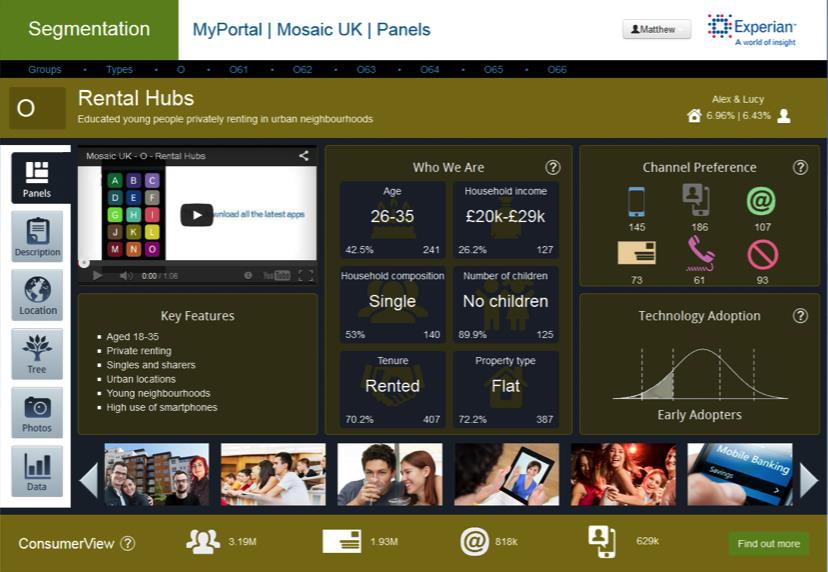
\includegraphics[width=\textwidth]{mosaic_segmentation_portal.jpg}
  \captionof{figure}{Segmentation portal visualising Mosaic data \citep{Experian2014}.}
\end{center}


		\subsection{IBM Cognos}
		
			\subsubsection{Introduction}
			
Addressing the need of businesses for software that helps to achieve a competitive advantage, IBM has a rich portfolio of analytics products. These include solutions in areas of predictive analytics, risk analytics, prescriptive analytics, enterprise performance management and business intelligence \citep{IBM2015b}. The majority of IBM products in BI belong to the Cognos family and include very specialized applications like "Cognos Supply Chain Performance Procurement Analytics" as well as general purpose tools like "Cognos Business Intelligence".

The solution used at CEC is IBM Cognos Business Intelligence 10.2.1 and it is a set of tools that significantly eases processes such as importing data from different formats (e.g. csv, xml, xlsx), combining relational and multidimensional data, generating reports (real time reports, drag-and-drop GUI, database queries in SQL and OLAP), scheduling and redistributing reports, publishing reports on multiple platforms and many more. Tools available at the CEC include: Report Studio, Query Studio, Analysis Studio.

The desired objective can be achieved using different tools, but some of them are better fitted for a specific purpose. Report Studio was designed with reports creation in mind, while Query Studio was optimized for creating and editing complex database queries. CEC has two types of instances of IBM Cognos - production and development machines, accessible under different URLs.

IBM Cognos BI is an enterprise class SOA platform \citep{browne2010ibm}. Its n-tiered architecture is made up of:
\begin{itemize}
\item The web tier - provides user sessions connectivity to applications
\item The application tier - load balancing and processing of requests, managing storage of customer application data
\item The data tier
\end{itemize}


\begin{center}
  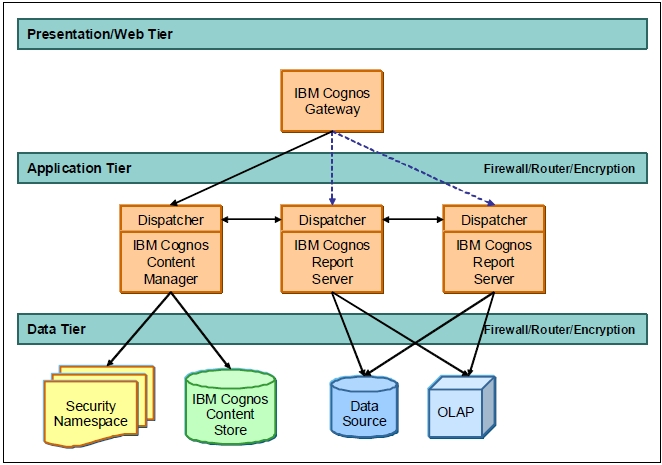
\includegraphics[width=\textwidth]{cognos_architecture.jpg}
  \captionof{figure}{IBM Cognos BI architecture \citep{browne2010ibm}}
\end{center}


The platform operates by using different services which are run at those three levels \citep{Browne2010}, for example:
\begin{itemize}
\item Agent service - responsible for running agents, "determines which tasks to execute and forwards those tasks to the monitor service for execution"
\item Monitor service - handles requests which will be run in the background including background tasks, reports scheduled to be run and e-mailed, jobs
\item Query service - "manages Dynamic Query Mode requests and returns the results to the requesting batch"
\end{itemize}
		
			
			\subsubsection{Working with IBM Cognos BI}
			
IBM Cognos can be accessed using either a web interface called IBM Cognos Connection or a Windows application. For the purpose of this project only the web interface was used.

\begin{center}
  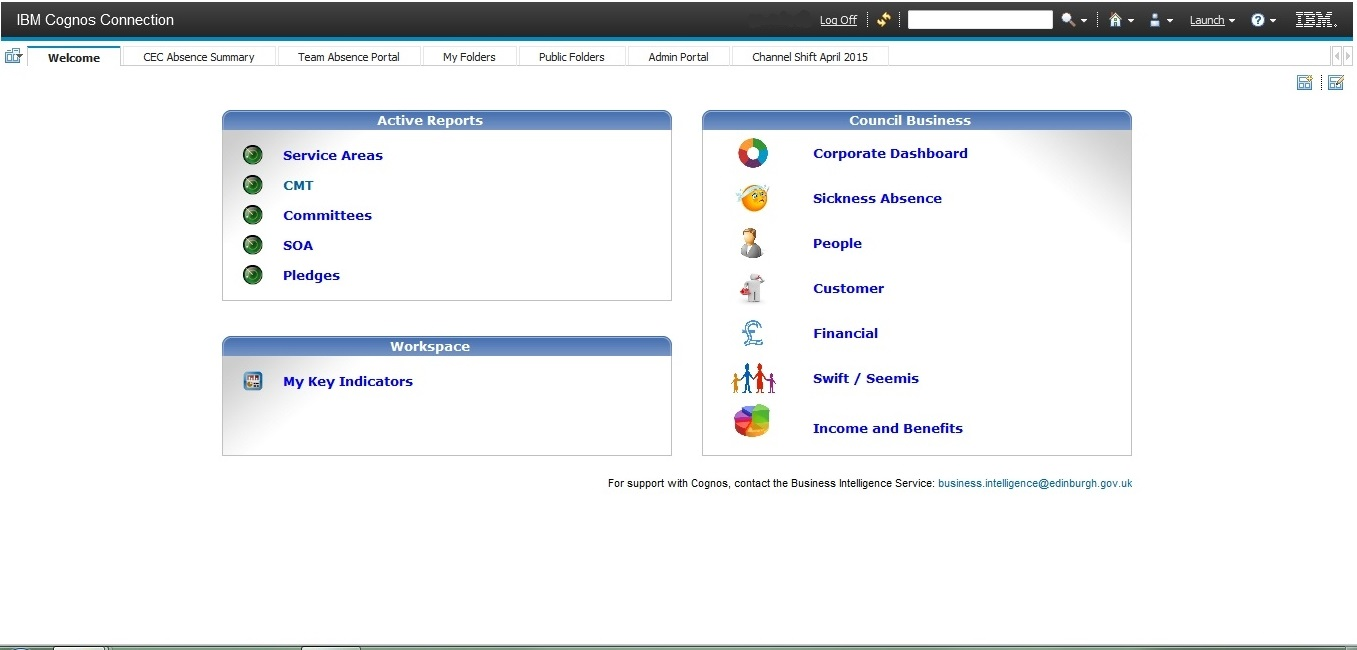
\includegraphics[width=\textwidth]{pre work/1st day Cognos - processed/welcome page of web interface of Cognos.jpg}
  \captionof{figure}{Welcome page of IBM Cognos Connection 10.2.1 (interface to all the tools available within your license)}
\end{center}


From this welcome page you can start applications available within your license, e.g. Report Studio. Selected activities that can be performed with the Report Studio include: creating data packages, creating and publishing reports and report templates.

Graphic User Interface (GUI) makes the entire process quick and easy, but it is used only to set the general structure of the report. The specifics, e.g. how to filter data, have to be implemented using queries.\\
Example of a filter:
\begin{lstlisting}
if ([No of interactions with CEC] > 3) then ( 'above 3') else ('up to 3')
\end{lstlisting}
Example of a counter:
\begin{lstlisting}
count(rows for [MW].[MW].[Date Created], [MW].[MW].[UPRN], [MW].[MW].[Subject])
\end{lstlisting}

Behind every report there is an SQL query which is run on the database by Cognos. They can also be saves as XML files. Below is an example of SQL query behind a single report:
\begin{lstlisting}
select 
       MW."Creation Source"  as  Creation_Source,
       MW."Group"  as  Group2,
       MW."Date Created"  as  Date_Created,
       MW."Reference #"  as  Reference__,
       MW.Subject  as  Subject,
       MW."Product Hierarchy"  as  Product_Hierarchy,
       MW.UPRN  as  UPRN,
       XCOUNT(MW."Reference #"  at MW.UPRN,MW."Reference #"  for MW.UPRN )  as  No_of_interactions_with_CEC,
       D_MosaicGroupType.GroupTypeCode  as  Group_Type_Code
 from 
       MW...MW MW,
       Mosaic.MosaicExport.dbo.D_MosaicGroupType D_MosaicGroupType,
       Mosaic.MosaicExport.dbo.F_MosaicAddresses F_MosaicAddresses
 where 
       (MW.UPRN = F_MosaicAddresses.Uprn) and 
       (D_MosaicGroupType.GroupTypeId = F_MosaicAddresses.MosaicGroupTypeId)
 group by 
       MW."Creation Source",
       MW."Group",
       MW."Date Created",
       MW."Reference #",
       MW.Subject,
       MW."Product Hierarchy",
       MW.UPRN,
       D_MosaicGroupType.GroupTypeCode
 filter 
       (XCOUNT(MW."Reference #"  at MW.UPRN,MW."Reference #"  for MW.UPRN ) > 3)
 order by 
       Date_Created asc
\end{lstlisting}

	\section{Define}
	
After the discovery phase an understanding of the specifics of the project within the Council has been achieved. The goal of the next phase was to narrow down the scope, find specific questions to be answered and make a decision about tools that would be used. Prototypes were created (simple reports) to prove the capabilities of the system. This phase ended with clear objectives and a general idea of technical aspects of implementing them.	
	
		\subsection{Preliminary work}
		
			\subsubsection{Meetings at the Council}
			
Figure 3.1 shows all people I interacted with in the entire project with those I spoke with in the Define phase marked with two ovals.

At this stage the clients were encouraged to drive the design decisions, e.g. they had a final say in selecting questions to answer with this project. This was mostly done in cooperation with Sally Kerr and Andy Thomson.

The meetings were also trying to select tools that would be used and if possible try to confirm they could be used by building a simple prototype. This was mostly done in collaboration with people from the BI section of CEC, namely Kevin Kelly and Angela McInnes.

Chris Jeffery provided insights about the CRM dataset.

Emilio G. Zamudio was another student of University of Edinburgh that was working on a project with CEC. During discussions with him I wanted to ensure that scopes of our projects do not overlap.
			\subsubsection{First iteration (proof of concept)}
			
The purpose of this stage was to go through the entire cycle of development. Before discussing what kind of analyses would be useful to the Council I had to confirm that it was possible to use the two datasets together and understand what limitations to the process were. There were no existing reports of this kind so I had to create a Cognos package for CRM and Mosaic data.

The Mosaic package has already been imported to the platform as it was being used in other Business Intelligence reports. The process of importing CRM data was manual, but it is planned to be automated in the future. It is assumed that UPRN uniquely identifies the user.

What I needed to do was to add to the Mosaic package an external data source (CRM dataset) using built-in Extract, Transform, Load (ETL) mechanisms, which required administrative access rights. The platform is quite flexible when it comes to file extensions and data formats. Some of the acceptable extensions include: .csv, .xls, .xlsx, .xml. The CRM dataset was extracted from the Council's system and saved as an .xlsx file on a shared network drive. I then created the package and generated a few simple reports as described below.

Figure 3.5 shows a simple chart created to confirm that it is possible to use both datasets together. Figure 3.6 shows numerical data behind that chart, verifying that entries are linked together properly using UPRN. Figure 3.7 is based on the same dataset, but a different dimension is used on axis.

\begin{center}
  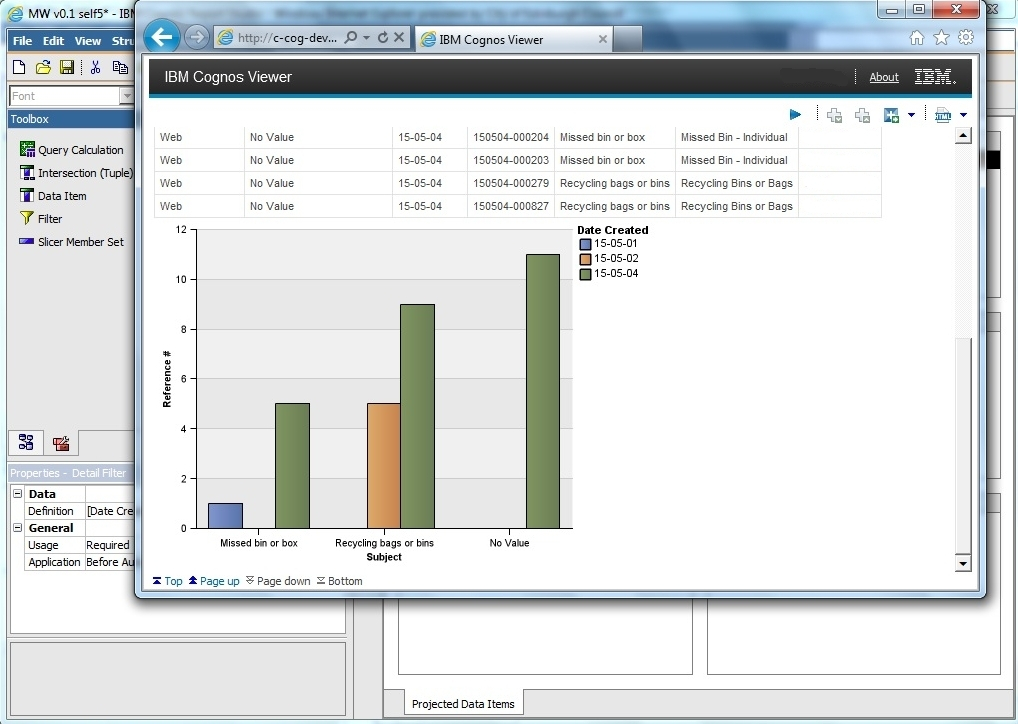
\includegraphics[width=\textwidth]{pre work/2nd day Cognos - processed/creating chart - first chart.jpg}
  \captionof{figure}{Simple chart created to verify capabilities of the tools used.}
\end{center}

\begin{center}
  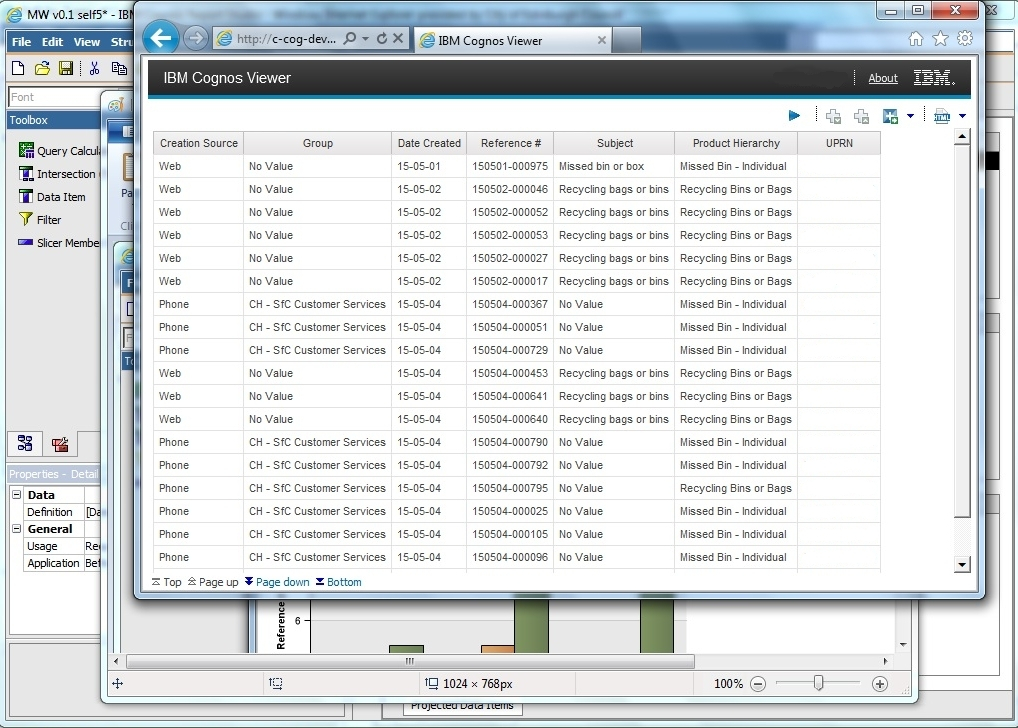
\includegraphics[width=\textwidth]{pre work/2nd day Cognos - processed/creating chart - first chart, data to confirm chart is valid.jpg}
  \captionof{figure}{List confirming that datasets are linked properly.}
\end{center}

\begin{center}
  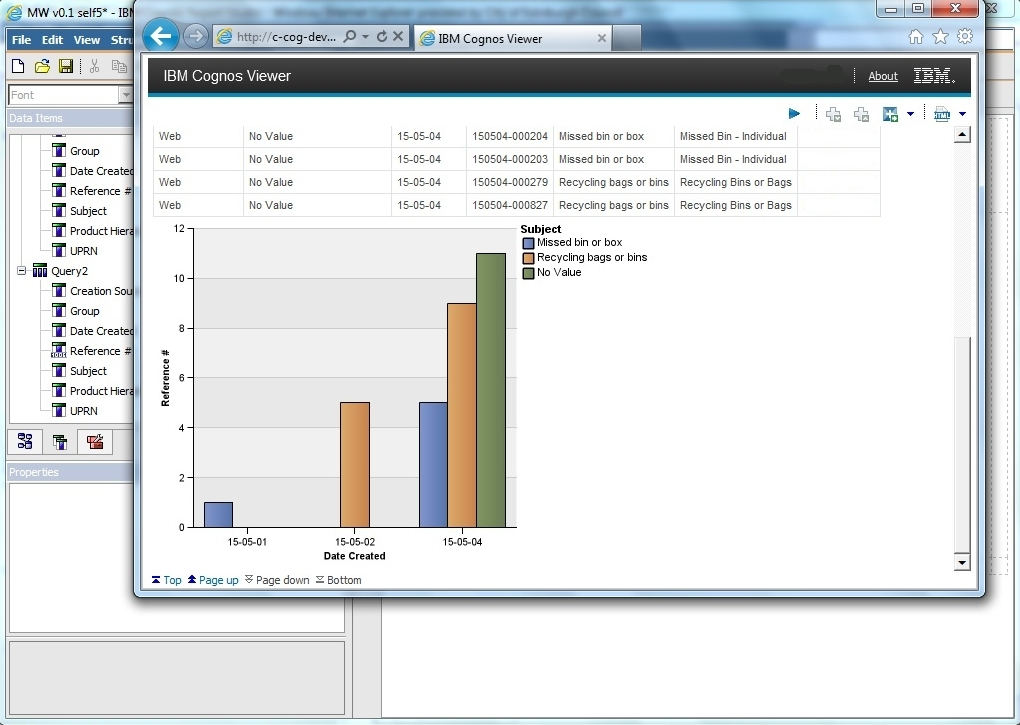
\includegraphics[width=\textwidth]{pre work/2nd day Cognos - processed/creating chart - first chart, other dimension.jpg}
  \captionof{figure}{Simple chart created using a different dimension of the dataset.}
\end{center}
\vspace{1cm}
A number of other charts were generated to further understand possibilities of the tools. Figure 3.8 is showing the use of CEC services in different Mosaic groups which are listed on axis x. Figure 3.9 is showing the same data as Figure 3.8, but uses Mosaic types which are more granular. Figure 3.10 covers only four services, which are the most widely used, namely "Missed bin individual", "Missed bin or box", "Recycling bags or bins" and "Recycling bins or bags".

\begin{center}
  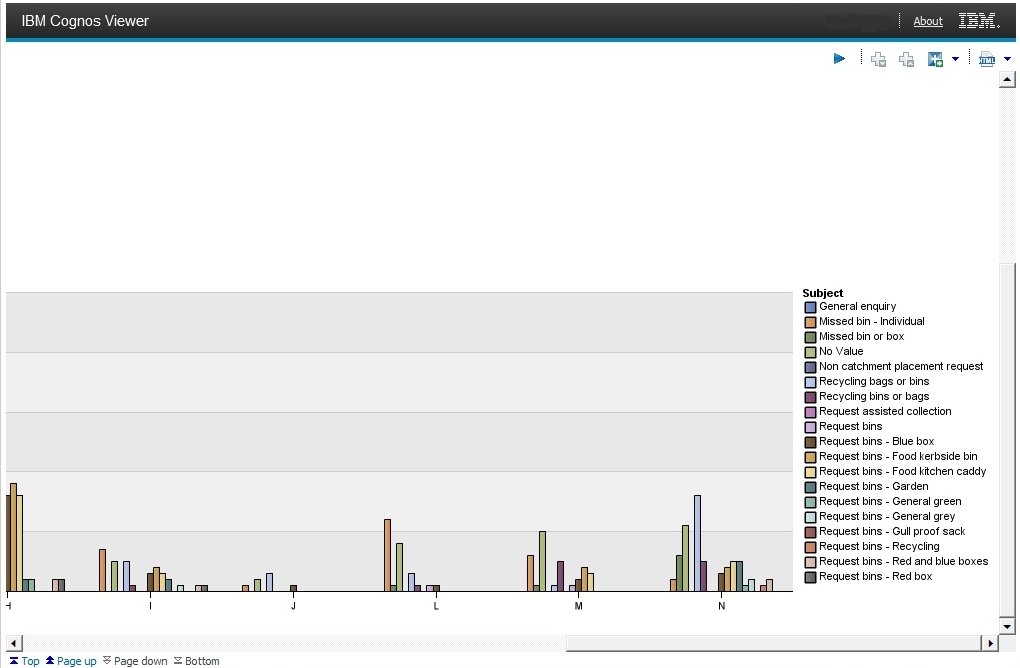
\includegraphics[width=\textwidth]{pre work/2nd day Cognos - processed/second chart, crm and mosaic, all subjects, entire May.jpg}
  \captionof{figure}{The use of CEC services across Mosaic groups.}
\end{center}

\begin{center}
  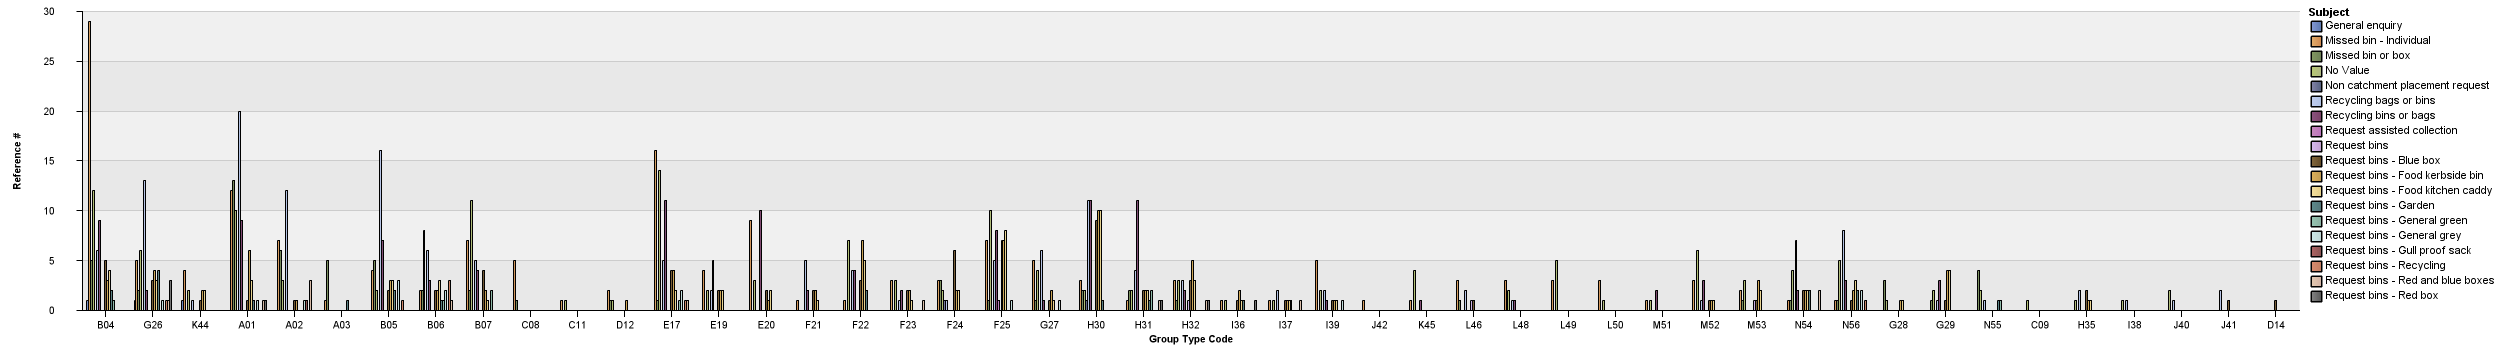
\includegraphics[width=\textwidth]{pre work/2nd day Cognos - processed/group code - all reports.png}
  \captionof{figure}{The use of CEC services across Mosaic types.}
\end{center}

\begin{center}
  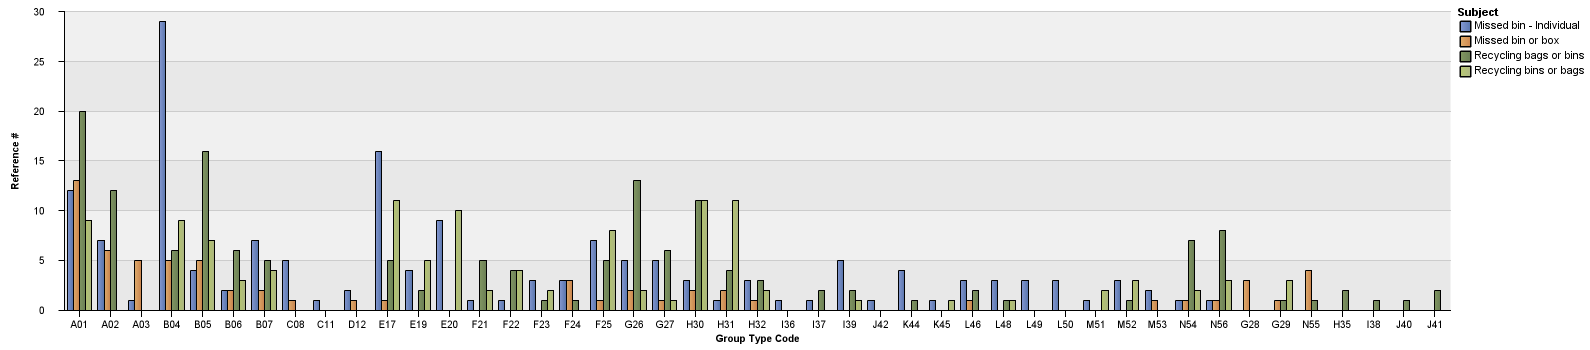
\includegraphics[width=\textwidth]{pre work/2nd day Cognos - processed/group code - bins, recycle.png}
  \captionof{figure}{The use of four most common services across Mosaic types.}
\end{center}


			\subsubsection{Selected problems}
			
Selected problems experienced in this phase are listed in sections below.			
			
				\paragraph{Linking problem}\mbox{}\\
During the import stage, where the CRM data was being added to the Mosaic package, there was a problem with linking the two datasets. As a result, I was considering alternative solutions in which I would build the necessary tools.

One of the analysed solutions included setting up a server with an SQL/NoSQL database, populating the database with the CRM and Mosaic data and then conducting analysis using Python. The focus of the project would shift and the insights generated would be of a different level and quantity. This would decrease usefulness of the project to CEC and move the project away from the initial objective.

After a couple of failed attempts with Cognos I wanted to go through the process step by step and document the problem in as much detail as possible and move on to building the new setup. I was using Cognos documentation in the process \citep{IBM2015, IBM2015c}. Fortunately, the detailed approach adopted has led to finding a solution and the platform could be used in the project.

\begin{center}
  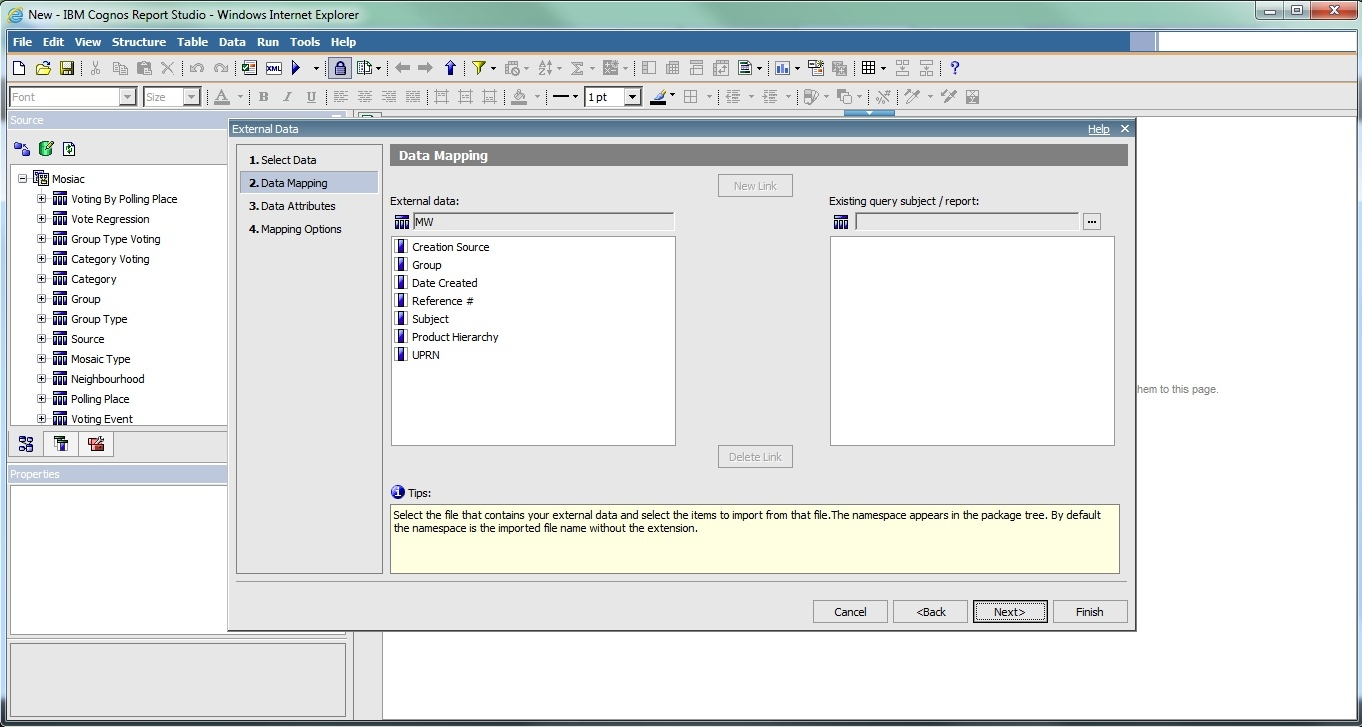
\includegraphics[width=\textwidth]{pre work/1st day Cognos - processed/importing CRM data into Cognos 2.jpg}
  \captionof{figure}{CRM data unavailable for linking with Mosaic package.}
\end{center}
	
				\paragraph{CRM data}\mbox{}\\
One of the problems with analysing CRM data was the quality of data. There are inconsistencies in implementations across different channels. For example, entries regarding requests for recycling bins or bags reported through two different channels had different values in the "subject" field: web - "Recycling bags or bins", phone - "Recycling bins or bags". Initially it was believed that it was an older implementation, but both values were present throughout the entire dataset suggesting both of them were in use. As a result, when analysing the data, filters had to include all possible strings related to the desired value or use a different field - "Product Hierarchy", as was the case with the final reports.

Another problem was related to the lack of documentation of the deployment of the CRM system and difficulties in talking to someone knowledgeable about it. I could not establish in a reliable way the difference between "Product Hierarchy" field and "Subject" field. In the "Incidents" table there are entries: "UPRN", "second UPRN", "UPRN 2" but they are not documented anywhere. In cases like this a "best guess" approach had to be used. 
				
		\subsection{Design of the solution}
		
The initial reports served as a learning experience during which I became more familiar with systems and narrowed down the objectives further. I also ensured I would have the necessary access rights before making a decision to pursue this direction.

One of the decisions I had to make regarded data analysis methods. The advantage of using IBM Cognos was a very good integration of many smaller tools (e.g. ETL) and techniques (e.g. changing dimensions of analysis) which made the whole process much more effective and less time consuming. Consequently, I would be able to conduct much more analyses that would present more value to the Council.

Selected advantages of using IBM Cognos in the project:
\begin{itemize}
\item it is a tool that can be easily accessed by CEC employees (e.g. in their web browser)
\item the results could be used by CEC employees in the future (they can feed my reports with other data extracts and conduct the same analysis on it)
\item they could be used as a starting point for future reports (they can go through my files to see how I did it, they can expand them adding or rearranging some parts of it)
\item the project would be in line with the strategic direction of development of the Council so I would be directly contributing to the efforts of the Council
\item the result would be within the CEC environment (no need to migrate my solution to CEC environment)
\end{itemize}

In terms of ideas for analysis, I developed a list of questions I thought were relevant from the perspective of someone implementing or improving transactions at the Council. I than discussed it with CEC employees (Sally Kerr and Andy Thompson), added their ideas and gave them the final word about which ones to implement. The result was a list of three questions and a decision regarding further direction.
		
		\subsection{Design brief}
This section is a "design brief" which is a starting point for the next phase. It consists of selection of tools to be used and specific objectives.

The data analysis will be conducted using IBM Cognos platform and it will use Mosaic Experian package combined with an extract of the data from the CRM system. The reports generated will not be of performance indicators nature, but will try to find data that can show behaviour of citizens manifesting in the data. They are not (primarily) intended as monitoring tools, but rather as ways of expanding perception of what is happening in service delivery. The three main areas that will be covered are listed below and they are described in detail in the following sections:
\begin{enumerate}
\item Cases of intentional use of multiple channels for the same issue
\item Patterns of behaviour across different channels
\item Better understanding of primary users of CEC services
\end{enumerate}
		
			\subsubsection{Report 1 - cases of intentional use of multiple channels for the same issue}
			
Analysis from Report 1 is aiming at identifying cases where citizens want to report an issue, but do not trust in it being handled the same way through different channels. Presumably, the reasoning behind such behaviour is that if many tickets are opened for the same problem, one of them will "get the job done". The underlying assumption is that entries in the CRM system will not be identified as related to the same problem and that time of delivery differs across different channels. It will be solved the quickest possible way, because if the process behind one channel has more resources available it will be handled quicker than with the process behind another channel.

The purpose of this analysis is not to provide evidence about the assumptions being right or wrong, but to verify if such behaviour exists among receivers of the Council services.
			
			\subsubsection{Report 2 - patterns of behaviour across different channels}
			
The purpose of analysis within Report 2 is to understand patterns of behaviour of citizens across many channels.

Some of the patterns that might be revealed include:
\begin{itemize}
\item The user initiated a service through a channel of preferred choice (e.g. web-form). However, after not hearing from the Council for some time, the user is unsure about the status of the process and uses a channel that is considered trustworthy (e.g. face-to-face) to confirm its state.
\item Many users try to report a missed bin over a web-form, but eventually use a phone to do it (which highlights an issue with a particular web-form).
\item The user tries to use a digital interface, but for some reason goes back to the old way of accessing the service
\end{itemize}	
			
			\subsubsection{Report 3 - Better understanding of primary users of CEC services}
			
Designing is a task that should be conducted with the user in mind and having an understanding of who is the primary receiver of the design helps tremendously. For this reason, designers use "personas" which make it easier to model how the user thinks or behaves. The more detailed and accurate information about the user one has, the  better design decisions one can make, which results in interfaces and services that better fit the needs of people.

The questions that will be answered within this part of work are trying to increase the understanding of users receiving Council's services. In particular, three user groups are recognised:
\begin{itemize}
\item never used CEC services
\item uses CEC services occasionally (defined here as having no more than three interactions with CEC)
\item actively uses CEC services (more than three interactions with CEC)
\end{itemize}

The analysis is trying to identify socio-economic backgrounds that users from all three groups have. Because CRM data contains only data about citizens who used CEC services it will not contain information about the first group. However, by determining who is interacting with CEC one can conclude who is not using those services. In other words, social groups that do not appear in the CRM dataset can be categorized into the first group.

Some of the questions that could be answered include:
\begin{itemize}
\item Who are the primary users in general?
\item Which social group has the most interactions regarding a particular service?
\item Which service is the most popular within a social group?
\end{itemize}

	\section{Develop}
	
The implementation stage of the project started with three objectives coming from the previous phase. Subsequently, three reports were generated to provide analysis in those areas.

Development started in a fresh environment. CEC provided me with a designated work space together with a laptop and all the access rights necessary for the implementation (access from the preliminary stage was revised and a different setup was used). Due to this, the IBM Cognos package containing Mosaic Experian and CRM data had to be recreated from scratch as described in the Define phase.

The process in all three cases was to design a technical solution first and then implement it. The solution, a generated report, would consist of a number of queries that would provide results necessary to answer a question or an intermediate step (in more complex cases) that led to the desired insights. For more information on stages in the report creation, please see Appendix A containing a list of files used in the process.
	
		\subsection{Report 1 - cases of intentional use of multiple channels for the same issue}
		
Report 1 is trying to provide evidence for existence of a specific type of behaviour where citizens report one and the same issue using many channels at the same time.

Proving such behaviour using solely data analysis is very difficult and should not be left only to an algorithm. One of the problems with this kind of analysis is that behaviour of people with different intents might manifest in the data in the exactly same way. The report might identify users with "scattershot" approach, but also group in the same category non individual users like landlords, who visit many sites and then report a bulk of issues or residents who struggled with submitting a web-form and were helped by a consultant over the phone.

It has to be stressed that this analysis is not trying to automatically mark people as "bad users", but instead bring attention of a service manager to cases of unusual uses of the system. They might be pointing to a number of issues such as different delivery times across different channels, lack of trust in digital channels, low effectiveness of a channel in addressing a user need. They should be analysed and investigated further and should be treated as initial influences for further improvement.

			\subsubsection{Technical design}
Query 1: gather all relevant data (do not include entries if channel is not specified) and add a counter for how many issues someone filed on one day\\
Query 2: filter results of Query 1 so that only people who reported more than one issue on one day regarding the same subject are left\\
Query 3: filter out from Query 2 cases with only one occurrence of such behaviour (of multiple issues regarding one subject reported on the same day)

			\subsubsection{Implementation}

\begin{center}
  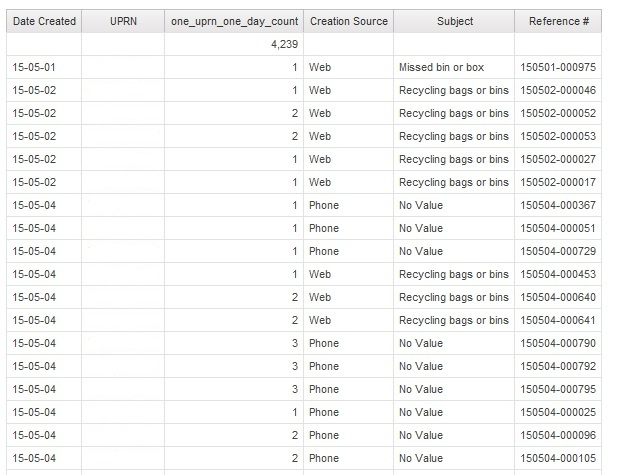
\includegraphics[width=0.9\textwidth]{Report 1/report 1, query 1.jpg}
  \captionof{figure}{Report 1, Query 1}
\end{center}

\begin{center}
  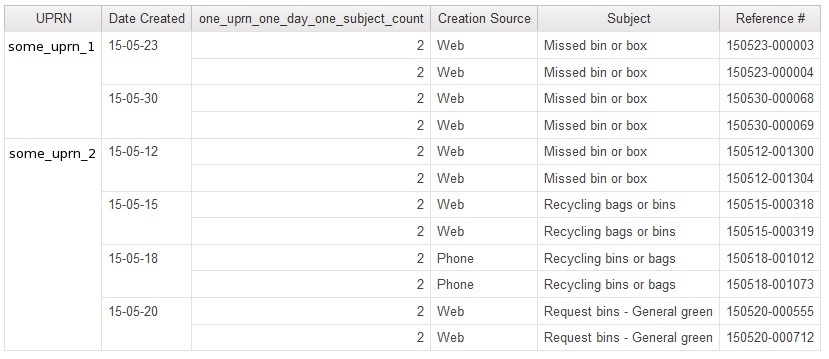
\includegraphics[width=\textwidth]{MW 12.08/MW 12.08/Report 1, query 3.jpg}
  \captionof{figure}{Report 1, Query 3}
\end{center}
	
			\subsubsection{Additional work}
			
There were only two cases found of residents reporting an issue over multiple channels over more than one day. It can be speculated that those were situations in which someone was having problems using CEC interfaces (cases of double entries with very short time distance).

In order to make the results easier to analyse, entries are grouped using UPRN - those coming from one user are listed next to each other. Within this group, they are ordered using reference number ("Reference \#"). The reference number is used instead of date of creation because there are multiple cases where there is more than one entry during a day. In those situations, ordering by the date does not ensure the same sequence as the sequence of creation. A reference number on the other hand, consists of two parts: the day of creation and a serial number assigned in an ascending manner and thus the original sequence can be deduced. In the following example, both reference numbers were created on the same day, but the second one was created later which can be determined by the second part of the string:
\begin{lstlisting}
150511-000837
150511-000849
\end{lstlisting}

In Figure 3.13, Citizen with some\textunderscore uprn\textunderscore 1 submitted a "Missed bin or box" through the web-form on fifth of May and made a phone call the next day regarding a service from the same "Product Hierarchy". It can be speculated, that both interactions were about the same issue. In order to verify such claim these interactions would have to be investigated further, e.g. using comments left by consultants (unstructured data) \citep{baars2008management}. Such additional information would be extremely useful in determining reasons for the user following up over the phone.

Citizen with some\textunderscore uprn\textunderscore 2 submitted two queries for the same issue on twelfth of May. The next day he submitted again two queries over the web for a different service, but what is really interesting is that after submitting them he made a phone call to the Council. This is a great example of identifying a situation where someone started with the web-form, but then for some reason made a phone call anyway. It might have been a simple question about the form, but clearly the person made the call after going through the web-form. It might be the case that putting on the form the information the user requested would help others.

Query 4 was created after conducting the above analysis. Its purpose was to provide a general overview on the number of multiple reports. This was to give an idea of how much people struggle with an interface and how quickly they learn it.

Query 4: count number of occurrence of such behaviour (how many times did someone report the same issue more than once on the same day)

\begin{center}
  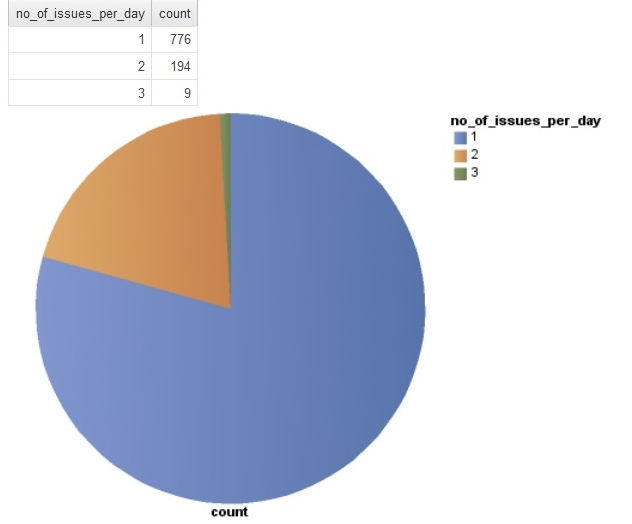
\includegraphics[width=\textwidth]{MW 12.08/MW 12.08/Report 1, query 4, cut.jpg}
  \captionof{figure}{Report 1, Query 4}
\end{center}

In simple words, there were 194 people in May 2015 who on two separate occasions reported on the same subject, on the same day.
			
		\subsection{Report 2 - patterns of behaviour across different channels}
		
Report 2 is trying to cast some light on behaviour of citizens across different channels.

It is based on two counters. The first one provides information about the total number of issues reported by a citizen ("count no of issues"). The second one counts the number of separate channels used to report those issues ("channels used"). Then, filters are used to remove from the report cases with the number of issues below two ("count no of issues \textgreater 1") and the number of channels used below two ("channels used \textgreater 1").
			\subsubsection{Technical design}
			
Query 1: count number of issues reported by a citizen, count number of channels used to report those issues, filter out number of issues below two, filter out number of channels used below two
			
			\subsubsection{Implementation}

\begin{center}
  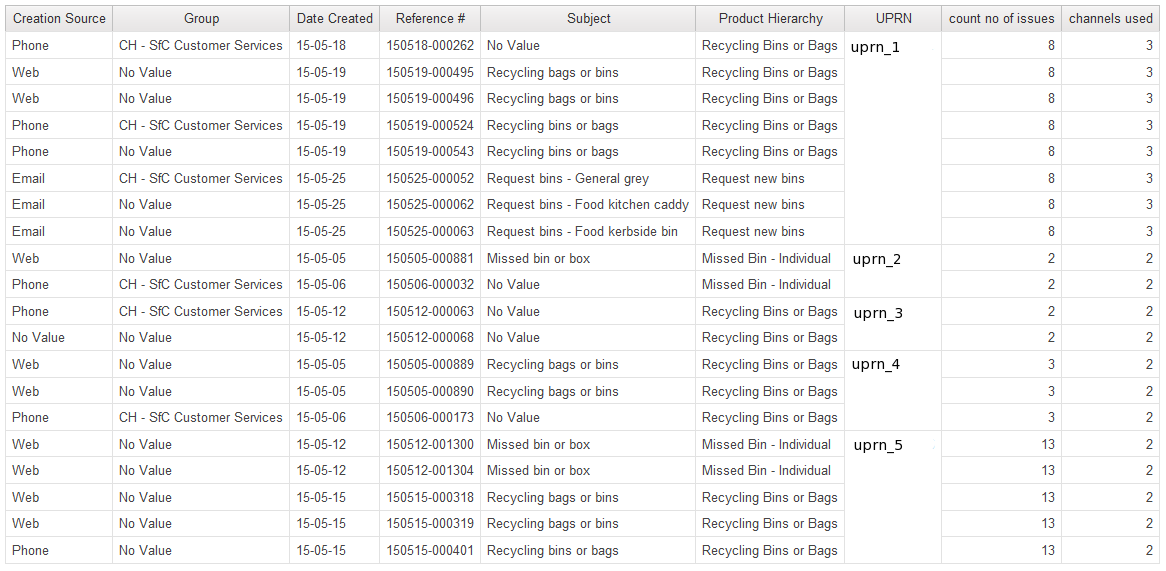
\includegraphics[width=\textwidth]{Report 2/report 2.2 page 2.png}
  \captionof{figure}{Report 2, example of results}
\end{center}

Figure 3.15 shows results of Report 2. Entries are grouped together using UPRN for simpler analysis. They can be interpreted by looking at creation source, reference numbers and "Product Hierarchy".
			
		\subsection{Report 3 - Better understanding of primary users of CEC services}
		
Report 3 starts from identifying users belonging to two categories as described in the Define phase, i.e. citizens who interacted up to three times with the Council and active users with more than three issues reported. After that, a series of queries are used in order to provide insights about socio-economic background of users.

The letters at the bottom of charts (A,B,C,…) are Mosaic groups. Detailed information about each group can be obtained using Mosaic Portal - Segmentation (as described in the Discover phase).

			\subsubsection{Technical design}
			
Query 1: gather relevant data, count number of all interactions of a user, assign a value based on the counter identifying the category as described above (up to three, above three), assign Mosaic groups to entries\\
Query 2: Which services are the most popular among people in both categories? - generate a chart with services on axis x, number of entries on axis y (counted by "Reference \#" field, count total aggregation) and data series for up to and below the threshold level\\
Query 3: Which Mosaic groups do people from both categories belong too? (which social groups use CEC services most actively) - generate a chart with Mosaic groups on axis x, number of entries on axis y (counted by "Reference \#" field, count total aggregation)\\
Query 4: Which services are being used by different Mosaic groups? - generate a chart with Mosaic groups on axis x, number of entries on axis y (counted by "Reference \#" field, count total aggregation) and data series for different services\\
Query 5: Which Mosaic group is the most active within a service? This part of the report is using "value prompts" which allow to select a service which will be analysed. It shows a chart for the selected service.
			
			\subsubsection{Implementation}
				
\begin{center}
  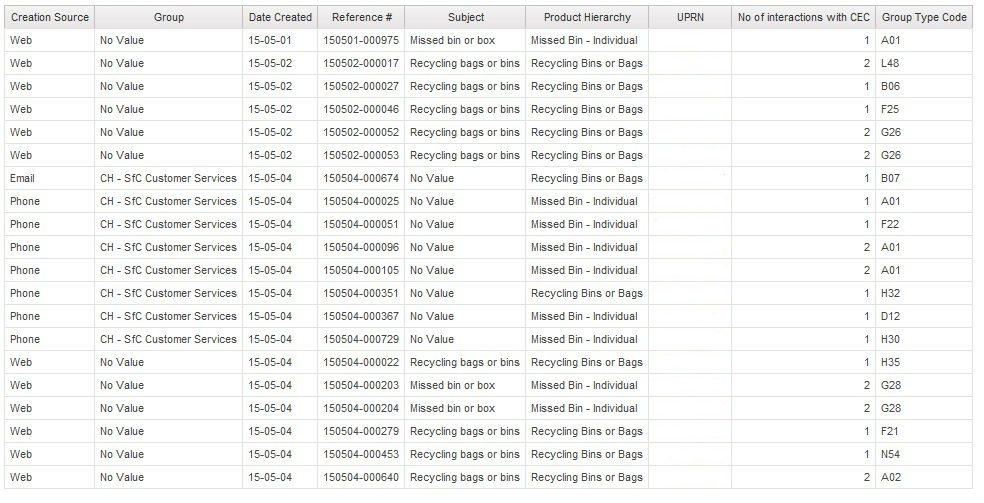
\includegraphics[width=\textwidth]{Report 3/list of citizens who had at most 3 interactions with the Council in May.jpg}
  \captionof{figure}{Report 3, Query 1 (up to three interactions)}
\end{center}

\begin{center}
  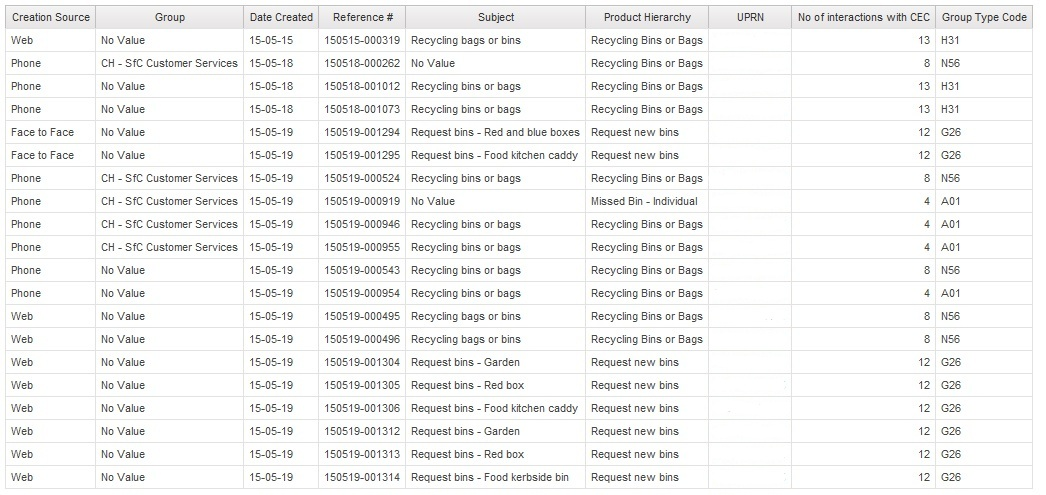
\includegraphics[width=\textwidth]{Report 3/list of citizens who had more than 3 interactions with the Council in May.jpg}
  \captionof{figure}{Report 3, Query 1 (above three interactions)}
\end{center}

Figures 3.16 and 3.17 are showing an excerpt of relevant data for the two user groups: citizens who interacted with the Council no more than three times and those who interacted more than three times.

In Figure 3.18 you can see on one chart the use of different services in both user groups. The same data is plotted separately in Figure 3.19 and Figure 3.20 for active users and occasional users respectively.

Such information is very important for someone responsible for a service. It gives them an understanding of the audience that they are addressing. It can be used when designing an interface such as a web-form or a mobile app, when preparing an information campaign or when inviting residents for participation in focus groups (to control demographics).

\begin{center}
  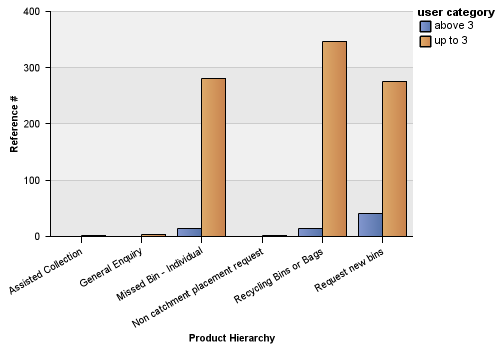
\includegraphics[width=\textwidth]{MW 12.08/MW 12.08/Report 3, query 2, axis sorted.png}
  \captionof{figure}{Report 3, Query 2}
\end{center}

\begin{center}
  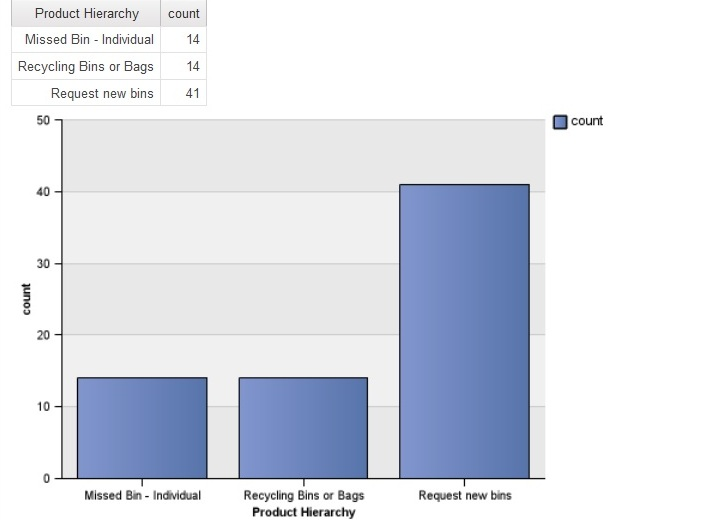
\includegraphics[width=\textwidth]{Report 3/report 3, 1.1.jpg}
  \captionof{figure}{Report 3, Query 2 (above three interactions with CEC)}
\end{center}

\begin{center}
  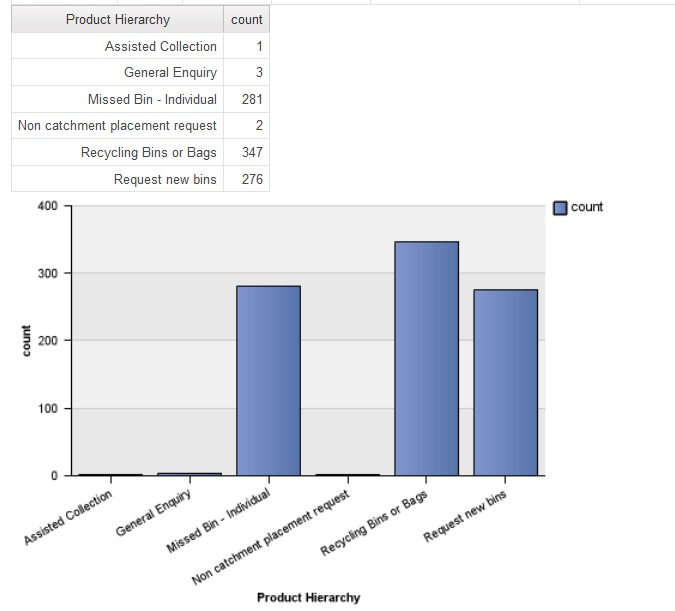
\includegraphics[width=\textwidth]{Report 3/report 3, 1.2.jpg}
  \captionof{figure}{Report 3, Query 2 (up to three interactions with CEC)}
\end{center}

Figure 3.21 is showing the distribution of the two user groups across Mosaic groups. Figure 3.22 and 3.23 are showing those categories separately. Based on these graphs one can tell that there are no regular users in Mosaic groups: C, D, J, K, L, M.  Very active groups include: A, B, G, H, N. 

\begin{center}
  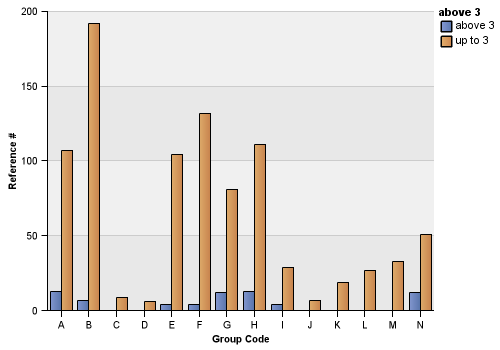
\includegraphics[width=\textwidth]{Report 3/report 3, 3.2 both on one chart.png}
  \captionof{figure}{Report 3, Query 3}
\end{center}

\begin{center}
  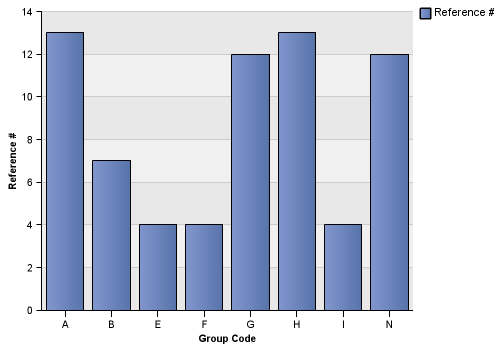
\includegraphics[width=\textwidth]{Report 3/report 3, 3.1 above 3.png}
  \captionof{figure}{Report 3, Query 3 (above three)}
\end{center}

\begin{center}
  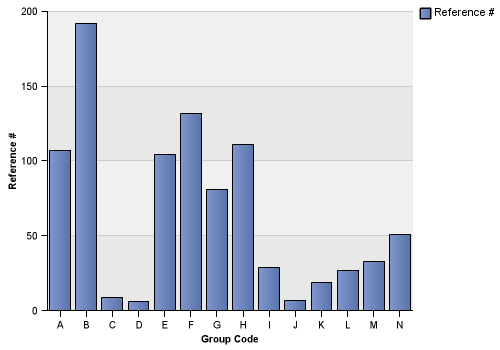
\includegraphics[width=\textwidth]{Report 3/report 3, 3.1 up to 3.png}
  \captionof{figure}{Report 3, Query 3 (up to three)}
\end{center}



\begin{center}
  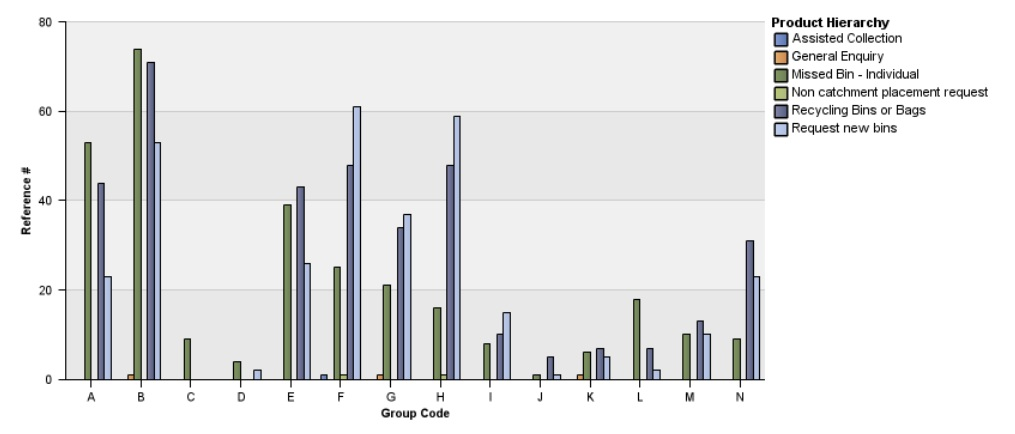
\includegraphics[width=\textwidth]{Report 3/report 3, 2.1.jpg}
  \captionof{figure}{Report 3, Query 4}
\end{center}

Figure 3.24 visualises the use of different CEC services across Mosaic groups. An example of an insight coming from this graph is that users from groups C and D are not requesting "Recycling Bins or Bags". Figure 3.25 visualises the same data with more granularity (using Mosaic types).

\begin{center}
  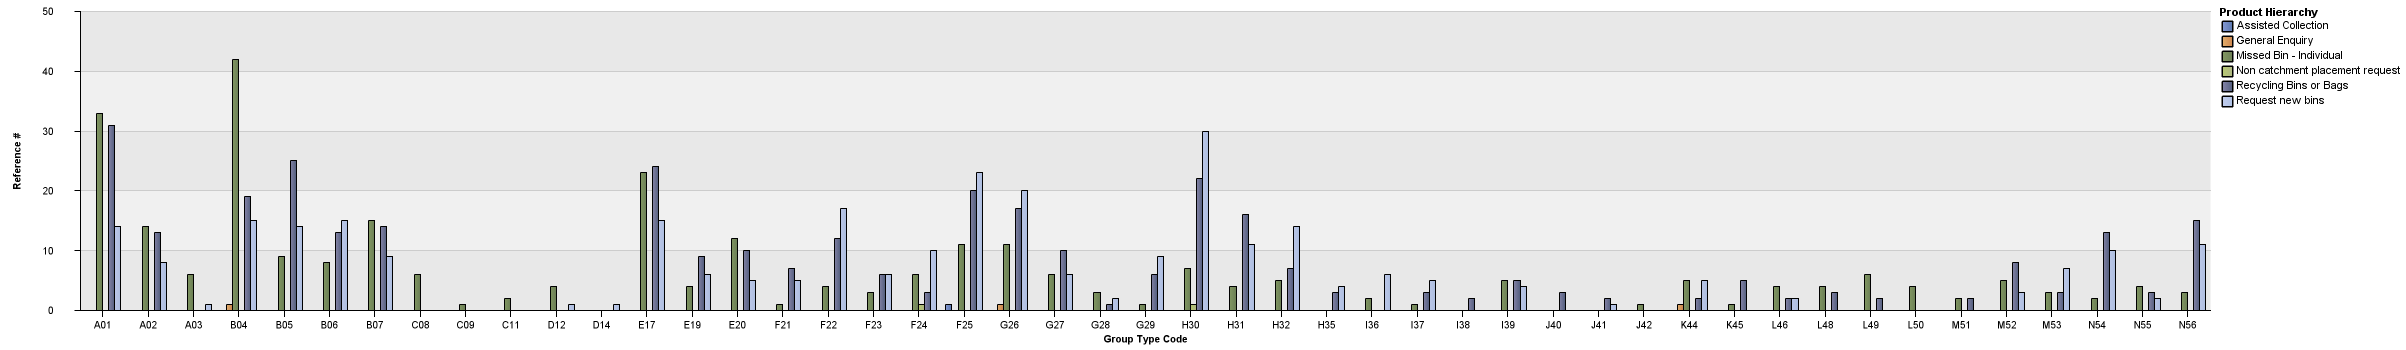
\includegraphics[width=\textwidth]{Report 3/report 3, 2.2.png}
  \captionof{figure}{Report 3, Query 4 (more granular, using Mosaic types)}
\end{center}

In order to make the analysis easier for a service manager, I created a report which accepts input from the user. After selecting a service from the drop down list, the corresponding chart is generated. Figure 3.26 shows the selection screen. Figure 3.27 shows a chart visualising the use of a service across Mosaic groups and Figure 3.28 provides more granularity by plotting the use across all Mosaic types.

\begin{center}
  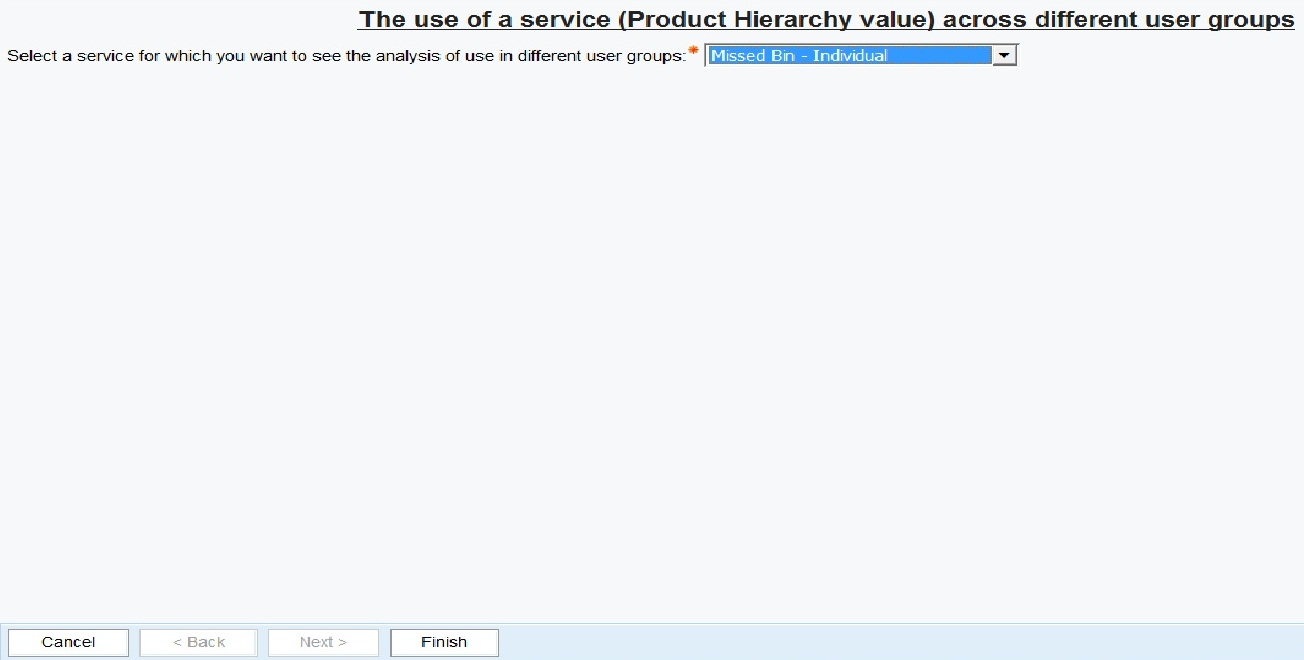
\includegraphics[width=\textwidth]{Report 3/report 3, 2.3 select screen, selected value.jpg}
  \captionof{figure}{Report 3, Query 5. Value prompt page with selected service - "Missed Bin - Individual"}
\end{center}

\begin{center}
  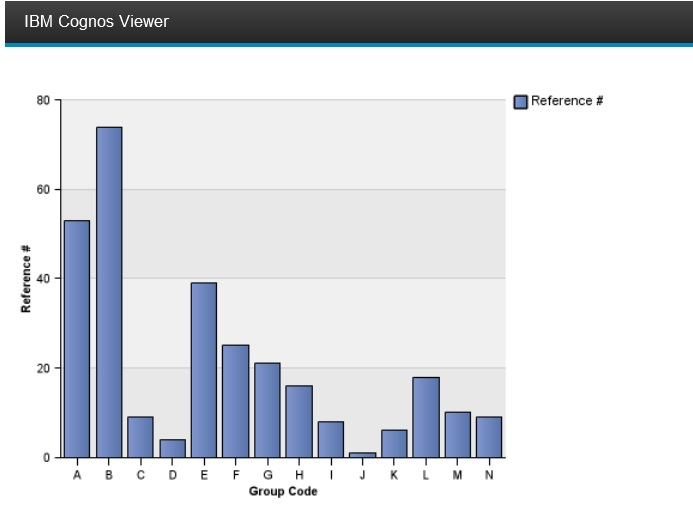
\includegraphics[width=0.75\textwidth]{Report 3/report 3, 2.3 group code chart.jpg}
  \captionof{figure}{Report 3, Query 5. The use of "Missed Bin-Individual" across Mosaic groups}
\end{center}

\begin{center}
  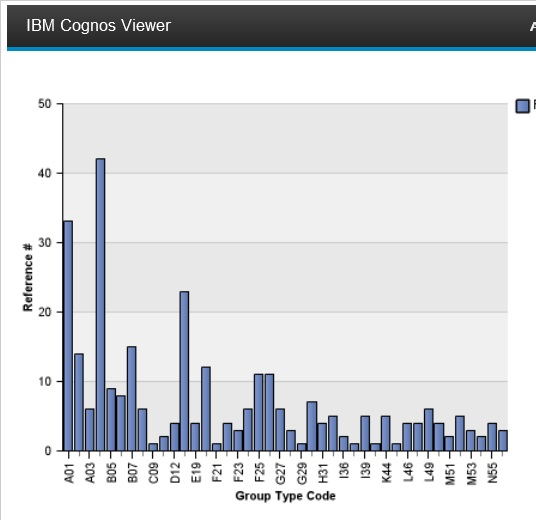
\includegraphics[width=0.9\textwidth]{Report 3/report 3, 2.3 group type code chart.jpg}
  \captionof{figure}{Report 3, Query 5. (more granular, using Mosaic types)}
\end{center}

	\section{Deliver}
	
		\subsection{Presentation at the Council}
		
In the delivery phase, I gave a presentation to CEC employees. The purpose was to present the project as a whole, show how to use the reports and evaluate their usefulness (receive feedback). Below are some quotes from the meeting in which Sally Kerr, Andy Thomson and Gosia Szymczak took part.\\\\
''It's very useful for us as well to have somebody coming from outside and giving us a fresh perspective and it is work that we have to continue with, so it's really interesting''\\
Sally Kerr\\\\
''One of the questions that we had, which obviously I think you didn't really have time to completely develop or it might be in your dissertation, was looking at (…) number of profiles we had and try to look at usage across those, because when we had originally done those profiles we made a best guess at the forms they would use the most. One of the questions was, did we get it right? (…) it would be very interesting to do that, because I think we are at a stage, moving with the new ICT supplier, to review that, to actually look at that model and then how is the supply going forward and also in terms of the communication campaign as well''\\
Sally Kerr\\\\
''We haven't been doing anything as in depth as that because nobody has asked us to do that. It's interesting just to see (…) the person is trying and trying to do it three times on the web and it's not going anywhere so there must be something.''\\
Gosia Szymczak\\\\
''I think the problem that we have (…) there is a bit of assumption with analysis there, which is very difficult to get away from unless you have user tests face-to-face (…) which I would recommend that we do, because however much (…) tracking tools, I still think you need to be going back to citizens just to actually make sure you are developing in the best way.''\\
Sally Kerr\\\\
''This is very interesting, just to get the indicators is very interesting and it's something we can share, it's just really important.''\\
Sally Kerr\\\\
''If a person is recording two or three times the same thing does that mean it's one complain or is it three complaints from the same person. It's helping us understand and analyse the stats, have a look at the stats, if the stats are correct, because there are three complaints from the same person on the same thing from the same address.''\\
Gosia Szymczak\\\\
''What we need is a good methodology for how you would do that (solve problems experienced by users), because we don't have the resource to give that kind one-to-one all the time (go through an individual problem), so this is really useful.''\\
Sally Kerr\\\\
''To be honest, we should be really carrying out this kind of analysis regularly to actually see if behaviours are changing. (…) That's a recommendation I would make, that we should be looking at how we do that for the future.''\\
Sally Kerr\\\\
''From University's point of view there are definitely opportunities, now we know how it all works for students to be involved with a particular piece of work if it's felt to be of interest. Working with BI on that, we will discover other areas that will be very useful as well.''\\
Sally Kerr

	\section{Problems}
	
In this part, selected problems experienced during the project are described. They are listed here in order to document the process as well as provide feedback for the design process:
\begin{itemize}
\item For a substantial part of the project, I did not have a pass to the building. It would be useful to have a starting date fixed in order to prepare a temporary pass and access rights for systems.
\item The fact that project had an open nature at the beginning was a very important part of it and helped in achieving a natural convergence between different teams of CEC and making the outcomes relevant and useful to the Council. However, this should not result in not having a clear business owner (e.g. Business Intelligence and Digital Service). Allocating even a small amount of resources (time of people involved) by senior management would help the project by not putting the burden of excessive time on CEC employees and would help in getting access to the licensed platforms within existing structures.
\item In order to work with ICT systems in the Council a workstation (from the Council) is required. It would help to use a laptop together with the account created for the temporary pass that would have all the necessary accesses. During the project, the use of a laptop had to be supervised (putting additional burden on CEC employees) together with an account that had extremely limited storage space.
\item Difficulties were experienced when creating charts using calculated fields (no problems using values from a database). Charts do not work with automated aggregation function, you have to use "none" as the aggregation function.
\begin{center}
  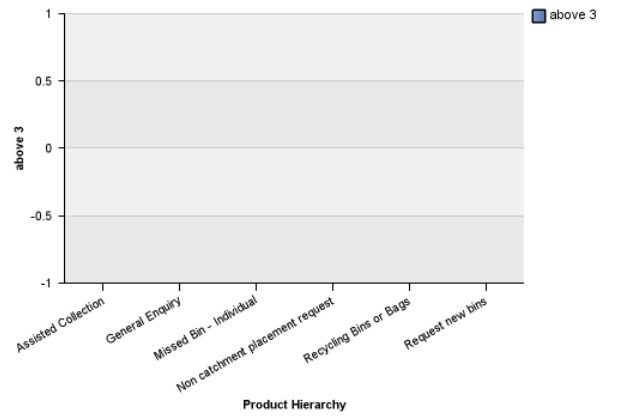
\includegraphics[width=\textwidth]{Report 3/report 3, chart 1, aggregation function not set.jpg}
  \captionof{figure}{Report 3, Query 2. Aggregation function not set to "none"}
\end{center}
\item The CRM data source file had blank entries. IBM Cognos considered them valid (did not filter them out). They were showing up in all analyses as empty and could not be filtered out. There was about 4200 of them. They were removed from the extract manually.
\begin{center}
  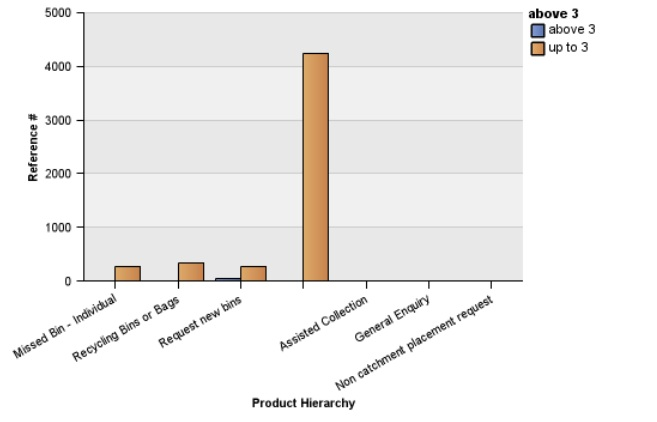
\includegraphics[width=\textwidth]{Report 3/data_source_problem.jpg}
  \captionof{figure}{Report 3, Query 2. Empty entries showing up in all analyses}
\end{center}
\item When a filter was implemented and then removed a result would be generated (different from when the filter was present). However, if the platform was restarted the results were different (for the same report).
\begin{center}
  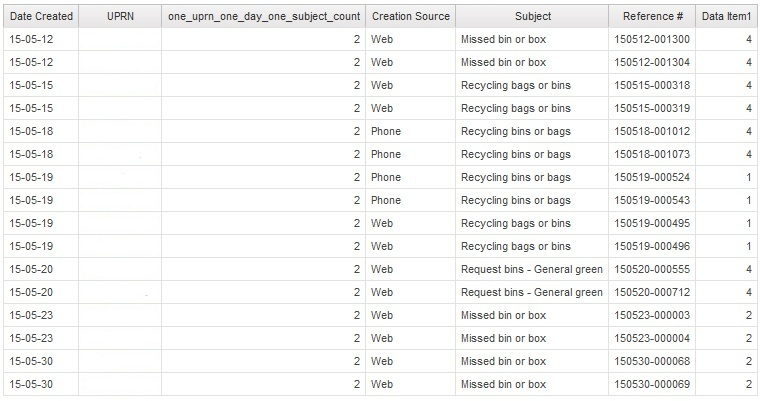
\includegraphics[width=\textwidth]{Report 1/problem.jpg}
  \captionof{figure}{Before restarting the platform.}
\end{center}
\begin{center}
  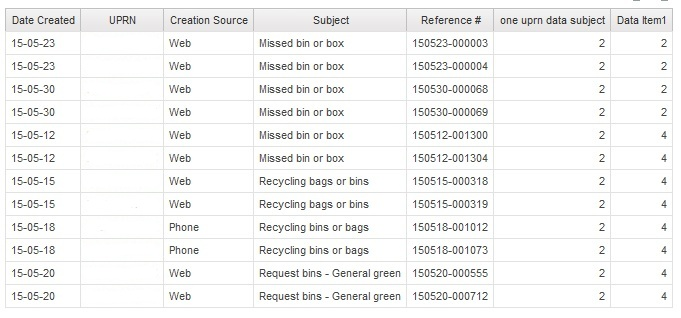
\includegraphics[width=\textwidth]{Report 1/report 1, query 3.jpg}
  \captionof{figure}{After restarting the platform.}
\end{center}

\end{itemize}


%% Sample chapter file, for use in a thesis.
%% Don't forget to put the \chapter{...} header onto each file.

\chapter{Analysis and evaluation}
	\section{Evaluation of the tools used}

		\subsection{CRM data}
		
The CRM data is easy to extract from the RightNow system and it is formatted in a way that can be read by Cognos to build a package. The "Incidents" table provides a very detailed picture of what is happening on every channel as entries are created even for queries where full data cannot be provided.

The "Incidents" table in the CRM system provides a lot of data for analysis, but is not sufficient to understand fully the situation around an interaction between a resident and the CEC. It would be extremely useful to combine it with analysis of unstructured data, e.g. comments left by consultants interacting with citizens.

The "Incidents" table in the CRM system contains only information about transactions initiated by citizens, e.g. they submitted a web-form. It would be very useful to combine this data with web analytics to widen the analysis and add cases where the form was not submitted, e.g. someone started filling the form, but for some reason did not submit it or made a phone call to the Council instead.

In Figure 3.13 (Report 1, Query 3) you can see that on 15-05-15 and 15-05-18 someone contacted CEC regarding a service belonging to the same "Product Hierarchy". However, they used different channels. As a result values in the field "subject" are different. This is probably due to inconsistencies in implementations between web and phone channel. This has an impact on the quality of data. 

The "Incidents" table in the CRM system does not contain a field that allows identification of all entries related to one problem. Up to my best knowledge there is no mechanism at the moment to link multiple "Incidents" entries regarding the same problem, e.g. many people reporting the same bin as missed. 

It was difficult to determine a number of things about the CRM system and data. It would have been useful if access to the documentation was provided or a person knowledgeable about the system could provide support.

The results of the project were greatly limited by resources, in particular by the time available. If there was more time available, it would be possible to review other tables in the database (instead of only relying on the suggestion of clients).
		
		\subsection{IBM Cognos}

Cognos is a very robust platform. It makes many steps in the development process smoother and provides very convenient channels for publishing. It deals well with ETL activities, i.e. exporting data from many formats and the initial processing of integrated data. With Cognos one can work with both relational and dimensional data at the same time, e.g. SQL and OLAP can be used on separate datasets and be combined in one report. It makes editing easier, e.g. changing a field in one part changes it everywhere else. There are free, learning resources available online - the official documentation, cookbooks, tutorials \citep{MIT}. However, some things are not very intuitive and you have to learn how to think about them "in Cognos categories". There are also many small bugs that have not been solved for a long time.

	\section{Evaluation of the work undertaken}
	
The work undertaken in this project by no means exhausts the objectives or needs at the Council. There are many improvements that could be done even to the reports themselves, e.g. drill through reports - user selects a service, a chart is displayed with columns showing use across Mosaic groups and clicking on a column opens another chart showing the use within types belonging to this group.

		\subsection{Report 1}
		
Report 1 was looking for evidence of a specific behaviour. Therefore, it was not an open question in its nature. The scope of the analysis was not being changed or expanded depending on the data. Instead, there was a set of metrics which described this behaviour and so the implementation was looking for very specific patterns in the data. The objective was achieved and the report generates a list showing desired information (occurrences of interactions which potentially could point to deliberate use of multiple channels for one issue).
		
		\subsection{Report 2}
		
Report 2 was more "exploratory". It was not looking for anything in particular, but rather was trying to cast some light on behaviour. As such, the data dictated the direction of this report.

After initial findings it was clear that the analysis would benefit a lot from adding other sources of data to Cognos. One idea included adding unstructured data, such as comments of consultants handling an issue. Although it was possible to point to unusual cases, the "Incidents" table was in many cases insufficient to provide definitive answers. It gives very detailed information, e.g. which interface citizens use and how, who uses them (which can help when controlling demographics in focus groups), but not details about the interactions regarding a particular issue. Another idea was to add web analytics data. The "Incidents" table contains only information about issues reported to the Council. If a user went to the website and failed to submit a web form it would not be picked up by the CRM system. This potentially leaves out a lot of information about negative experiences of users.

Considering the above, this report in no way exhausts the topic and there are many questions to be answered. It might point a service manager to specific cases, but they require further analysis.
		
		\subsection{Report 3}
		
The third report was the most complex one. The objective, which was to show who primary users are, was achieved to the extent possible using Cognos. A number of charts were created showing the usage among citizens from different perspectives, giving a general overview and a detailed insight into specifics. It visualises the use across all services and the use of a specific service in different social groups. After viewing the charts, the information about social groups can be interpreted using the Mosaic portal (Segmentation), e.g. read the description of A01 group. The Mosaic package allows creation of charts with metric specific information, e.g. age distribution among users. However, the Mosaic personas (linked with CRM data using UPRN) are descriptions of households, not individuals. Having that in mind, the objective from the Define stage was to create a full picture using personas rather than analysing one attribute (it is not a single person reporting an issue, but a household).

	\section{Evaluation of methodology used}

The double diamond approach seems to reflect very well the dynamism of real life projects. The model describes "a rhythm of activities" that comes naturally. It includes a very open, exploratory first stage which leaves space for flexibility in adapting to what would be useful to the client.

The Discovery phase was extremely helpful in understanding the context of the problem and establishing ground before the next phases. Having such an open attitude requires a lot of persistence. The responsibility for the entire project rests on the designer and this causes "a creative stress". In the early stages, it is desirable not to be limited by having a concrete idea of what to do in the project (which is not the same as lacking any plan of action). The designer is exposing himself to the unknown and at many points the project could completely change direction or a path could be closed unexpectedly. It is critical to maintain composure, agility and be able to quickly adjust to the new conditions. It is also important to mention that it exposes the project to the goodwill of people across the entire organisation. The more the involved people are open and willing to help the better the outcome of the project will be. In terms of this particular project, the Council employees were very helpful and open-minded and their support has helped tremendously.

The three objectives that came from the Define phase (design brief) were developed in close cooperation with the beneficiaries (and at the same time the requesting party).

The Develop phase managed to address all questions from the previous stage. Having clear, measurable objectives, which were thought through, helped in planning the rest of the process and designing the technical aspects of it. The extent to which implementations were able to solve those problems was described in sections above (4.2 Evaluation of work undertaken).

The key outcome of Deliver stage was feedback from clients. It was very helpful to understand the extent to which it addressed actual needs and whether it succeeded in contributing to the on-going efforts in the Council (being in line with the current ICT strategy at the Council).
%% Sample chapter file, for use in a thesis.
%% Don't forget to put the \chapter{...} header onto each file.

\chapter{Conclusion}

Out of this project come many open questions and potential for further study. This dissertation gives a lot of details about the context of the project which were not available before. They can be of significant help in future endeavours.

The double diamond approach was particularly good at enabling cross department activity and flexibility in adjusting the scope of the project to the needs of the Council. Given the experience gained, a further study could try and evaluate different methods used at each stage of the process.

It is also important to stress that such projects are agile in nature and depend heavily on the organisation in which they are run, i.e. on the knowledge of people involved and their willingness to share it. This project is a great example of how open-mindedness of employees can help.

The timescale of the project was extremely short given its complexity. Many parts of it could easily take months to be properly developed. However, it was not aiming at delivering a fully-fledged product. Instead, the objective was to help the Council with evaluating new ways of thinking and working and looking at the design process in its entirety. As a result in many cases compromises had to be made.

BI reports like the ones generated in this project, should be treated as part of a bigger "transformation" project. Identifying cases where users struggled with a web interface by CRM data analysis should be one of many tools in the repertoire of a service manager. For example, they can be used to identify the demographics of people to invite for participation in a focus group.

Reports like these often raise further questions, e.g. when conducting analysis other things start emerging which could be objects of investigation themselves. There is a vast amount of possible insights coming from the CRM data.

The reports can be used by CEC employees on other data sets (it is a matter of pointing to a different source file). 

Coming up with insights and recommendations is only one step. Another question is how to manage a change in an organisation in order to benefit from those analyses. Ability to adapt to user needs and learn from the feedback is actually executed when such insights are followed by tangible actions such as a decision to deploy a change or a confirmation that current efforts are not misplaced.
%% ... etc ...

%%%%%%%%
%% Any appendices should go here. The appendix files should look just like the
%% chapter files.
\appendix
\chapter{List of files created during the project}

Files created up to Development Phase:
\begin{itemize}
\item “MW v0.1 self” - file to learn Cognos, shows how to combine CRM data with Mosaic data
\item “MW v0.1 self2” - first attempt to create a chart, doesn't work
\item “MW v0.1 self3” - attempt to create a chart, the query itself is working (everything is correct from the sytax point of view), but data is unavailable (aggregate function? filtering error?)
\item “MW v0.1 self4” - debugging the self3 report, added a list to show filtered data returned from the query. Result: there are some entries after filtering, but not as expected
\item “MW v0.1 self5” - from the start, this time the results are as expected (type of result, number of result)
\item “MW v0.2, working chart, 3 days, type of report – day” - first chart working as expected, it shows numbers about queries from all services grouped into Mosaic groups, counted by reference, limited to 3 days (x - mosaic group, e.g. B, G, K; y - count by reference, multiple columns - different values in 'subject')
\item “MW v0.2, working chart, entire May (previous was 4 days), Mosaic group – subject” - second chart working as expected, more accurate; x - type code, e.g. A01, A02; y - count by reference; only 4 services - 4 columns; for the entire May
\item “MW v0.2, working chart, entire May, Mosaic group – subject” - similar to previous one, not as detailed, x - Mosaic groups, e.g. B, G; y - count by reference; columns - different services (different values in 'subject'); entire May
\end{itemize}

Files created during the Development phase:
\begin{itemize}
\item “MW one issue on multiple channels v1.0” - find cases of misuse of multiple channels
\item “MW report 3”, “MW Report 3, blank chart” - base report that can be used to generate different reports about number of interactions with the Council, couldn't overwrite the original one, created another one to have a more meaningful name
\item “MW report 3, chart 1” - both above and below 3 interactions on one chart
\item “MW report 3, chart 1.1 blank” - template for the charts 1.1 and 1.2
\item “MW report 3, chart 1.1” - chart with only above 3 interactions, using filter
\item “MW report 3, chart 1.1 correct” - chart with only above 3 iteractions, using filter and a list to show data (identical to the previous one, extended with the list, couldn't overwrite the previous one)
\item “MW report 3, chart 1.2 correct” - chart with only below 3 interactions, with list
\end{itemize}
 
further parts of report 3 have 2 dimensions with many entries. As a result it would have a lot of columns and would not be easily readable. I decided to split it into 3 charts: groups x services; detailed groups x services; selectable service -> group

\begin{itemize}
\item “MW report 3, chart 2.1” - Mosaic group x services
\item “MW report 3, chart 2.2” - Mosaic group detailed x services
\item “MW report 3, chart 2.3 group code” - the use of the selected service across different Mosaic groups
\item “MW report 3, chart 2.3 group type code” - the use of the selected service across different Mosaic detailed groups
\item “MW report 3, chart 3.1” - blank report that is used as a basis for the other 3.1 reports
\item “MW report 3, chart 3.1 above 3” - Mosaic groups that active users belong to
\item “MW report 3, chart 3.1 up to 3” - Mosaic groups that occassional users belong to
\item “report 3.1 “- 3 charts on one page
\end{itemize}

Another session:
 
\begin{itemize}
\item “MW Report 2, 2.1” – identify citizens who interacted multiple times
\item “MW Report 2, 2.2” – multiple interactions through different channels
\end{itemize}
 

\include{appendix2}
%% ... etc...

%% Choose your favourite bibliography style here.


%% If you want the bibliography single-spaced (which is allowed), uncomment
%% the next line.
% \singlespace

%% Specify the bibliography file. Default is thesis.bib.
\bibliography{thesis}

%% ... that's all, folks!
\end{document}
